\part{Results}\label{part:results}

\section{Verification problems and references}\label{sec:res:setup}

\textbf{Problems.} All results use two problems built in \code{examples/rmc/problems.py}, both with
\emph{matched physics} (no unresolved-resonance probability tables, stationary target for every
nuclide with $A>1$ above $10^{-6}kT$, nearest-temperature data at 294 K), so that the elastic
evaluator is exact and the reference Monte Carlo has the same physics:
\begin{itemize}
\item \textbf{Infinite medium}: 3.1\%-enriched UO$_2$ and graphite homogenized in a reflective box,
  one source region. It has no spatial residual at all, so it isolates spectral and kinematic
  effects, and its backward flux has the closed form $q(E')/\Sigma_t(E')$.
\item \textbf{Graphite pincell}: a UO$_2$ pin (radius 0.4096 cm) in graphite, pitch 1.26 cm, height
  2 cm, reflective on every face; a $12\times12$ source-region mesh gives 172 regions. CASMO-8 groups;
  random ray with 500 rays per batch and 500 batches (300 inactive); $k^{\mathrm{MG}}=0.64257$.
  Graphite without S($\alpha,\beta$) is unphysical but a consistent CE model for both methods.
\end{itemize}
The pincell is strongly under-moderated (the pin occupies a third of the cell, and graphite needs
about 115 collisions to thermalize a neutron), so its spectrum is hard: the flux per unit lethargy
peaks near 1 MeV, fast fission in U-238 matters, and $k\approx0.64$.

\textbf{References.} Every layer is compared with something stock OpenMC computes independently: the
uncollided flux of the field as a fixed source (\code{CollisionFilter([0])}), first-collision
production (\code{CollisionFilter([1])} in one-batch eigenvalue runs, so that fission neutrons are
banked rather than transported), flights from the field's own weighted sample, and finally OpenMC's
eigenvalue calculation. Appendix~\ref{app:gates} lists the gates.

\section{Components}\label{sec:res:components}

\subsection{The field and the backward flux}

\begin{figure}[t]\centering
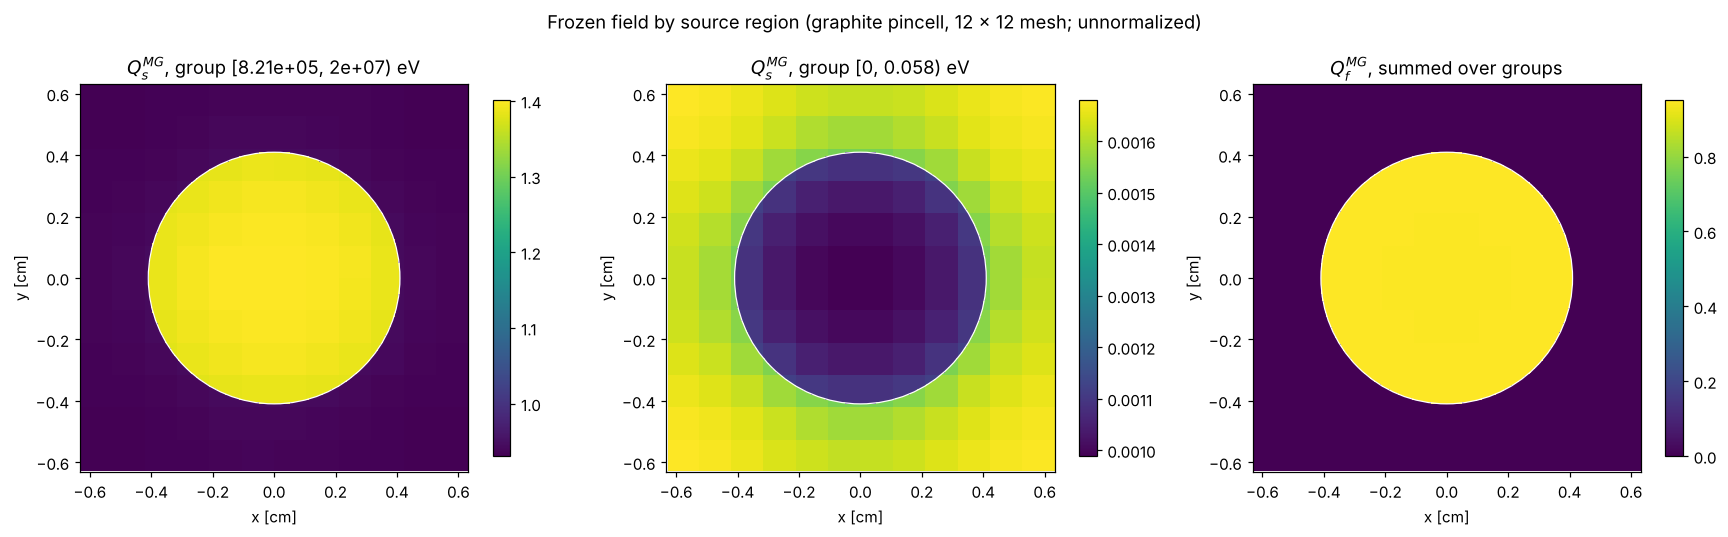
\includegraphics[width=\textwidth]{figures/field_maps.png}
\caption{The pincell's field: MG emission by region for both tags and a few groups. Fission emission is
confined to the fuel; scattering emission is largest in the graphite at low energy and in the fuel at
high energy.}\label{fig:res:field}
\end{figure}

\begin{figure}[t]\centering
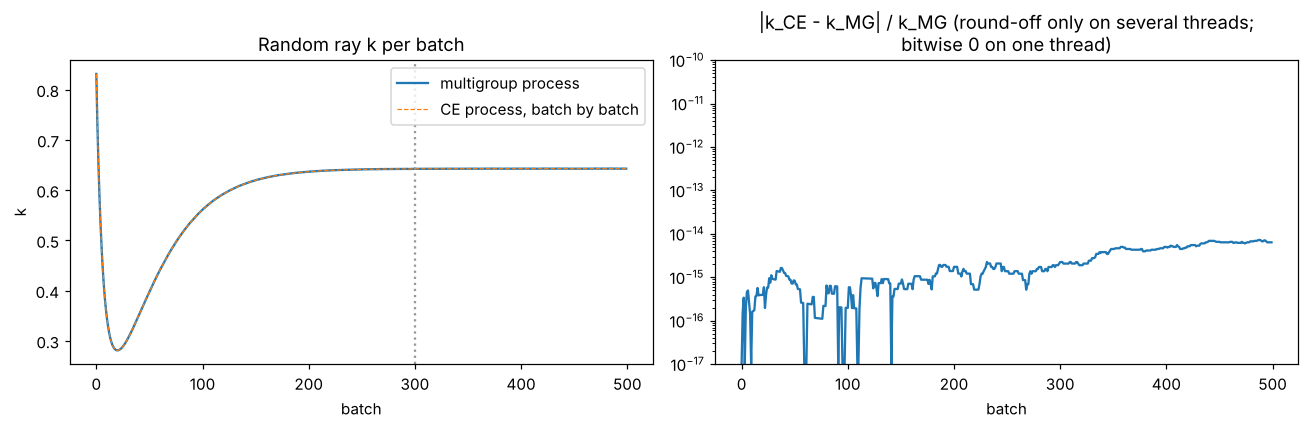
\includegraphics[width=\textwidth]{figures/ce_vs_mg.png}
\caption{CE against MG backward flux on identical paths. The two agree where the MG cross sections
represent the CE ones (smooth ranges) and differ inside resonance groups, where one MG $\Sigma_t$
averages a factor of $10^3$ of variation: this difference is what the MG control cannot remove.}\label{fig:res:cevsmg}
\end{figure}

Figure~\ref{fig:res:cevsmg} is the key picture for the control variate. Along a single path the MG
and CE fluxes share the geometry and the source, and differ only through the cross sections. In
groups where the CE cross section varies little the two fluxes are almost identical, so the MG flux
removes the path's directional noise. In the resonance group (4 eV to 5.53 keV) the CE flux depends
on the exact energy relative to the U-238 resonances, and no single group constant follows it.

\begin{figure}[t]\centering
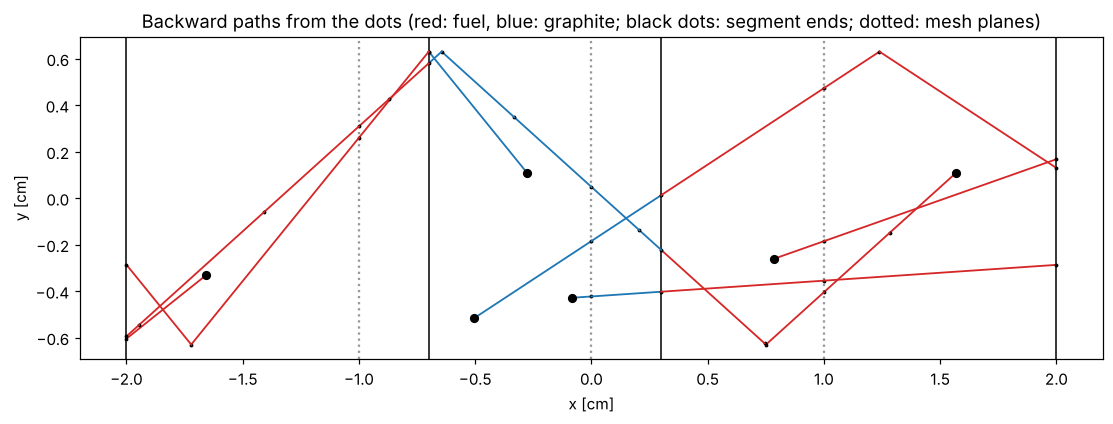
\includegraphics[width=\textwidth]{figures/tracer.png}
\caption{Backward traces through the pincell's source-region mesh and reflective faces, coloured by
region, against the analytic unfolded paths (G2.1): the tracer reproduces lengths, materials and
regions to $10^{-10}$ cm.}\label{fig:res:tracer}
\end{figure}

\subsection{Residual against first-collision tallies}

\begin{figure}[t]\centering
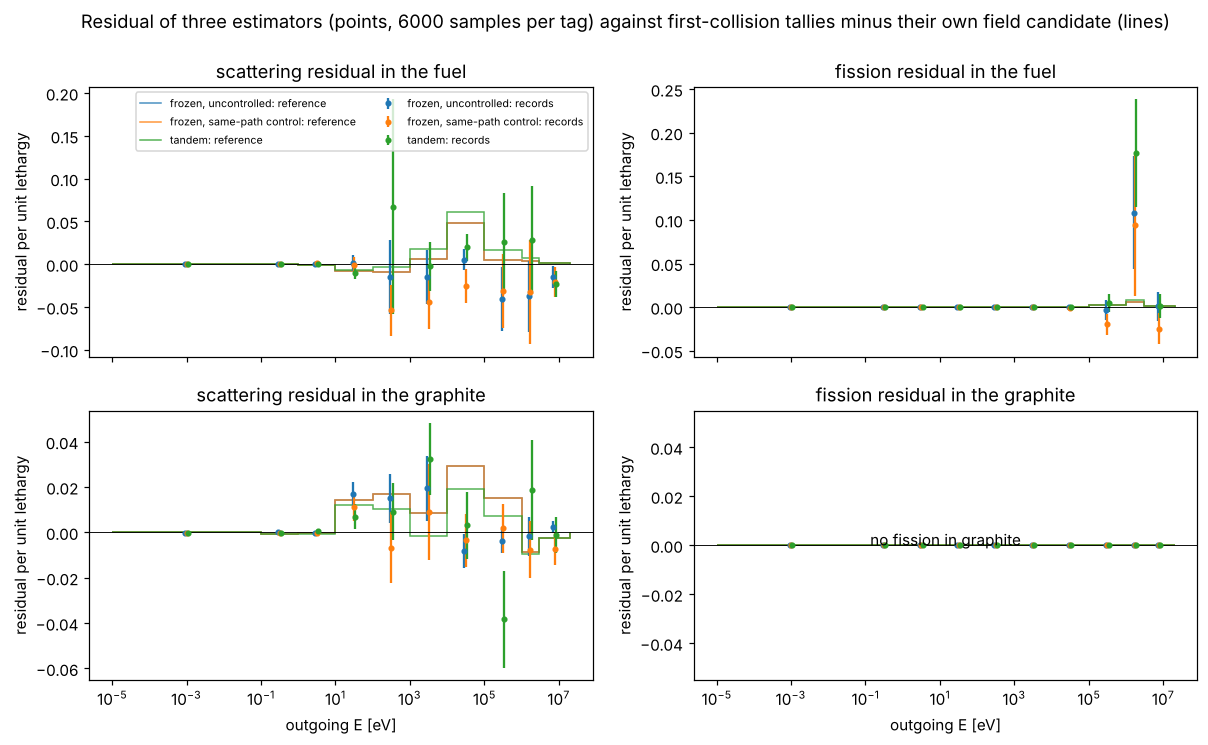
\includegraphics[width=\textwidth]{figures/first_collision.png}
\caption{The residual of the pincell's field by material and outgoing energy: OpenMC's first-collision
production minus the field integrated exactly (black) against several estimators (G4.1, G4.2). All
agree within statistics; their error bars differ by orders of magnitude.}\label{fig:res:fc}
\end{figure}

The residual is small: a few per cent of the production in any bin, largest in the fuel's epithermal
range (resonances) and in the fission spectrum (Figure~\ref{fig:res:fc}). Every estimator of
Table~\ref{tab:family} passes this gate, as do the density-free variants.

\section{The controlled residual study}\label{sec:res:controlled}

\subsection{Setup}

On the pincell with prescribed exact volumes, ten variants (Section~\ref{sec:classes}) were run with
$N=40{,}000$ samples per tag and compared, bin by bin, with a reference residual built from
$2.4\times10^7$ forward flights of each field component (a uniform point, a group in proportion to
the region's emission, a log-uniform energy within the group, weighted by $4\pi V\,q/p$), minus the
field integrated exactly. Three binnings: 36 logarithmic outgoing-energy bins per material; the 172
regions; and the radial cosine $\mu_\rho=\vO\cdot\mathbf e_\rho$ of the outgoing direction in each
material and energy range. Scans of $K$, common numbers, $J$, $M_{II}$ and the roulette cutoff used
$N=10{,}000$. All variants share their destination stream.

\subsection{The residual in energy, space and angle}

\begin{figure}[p]\centering
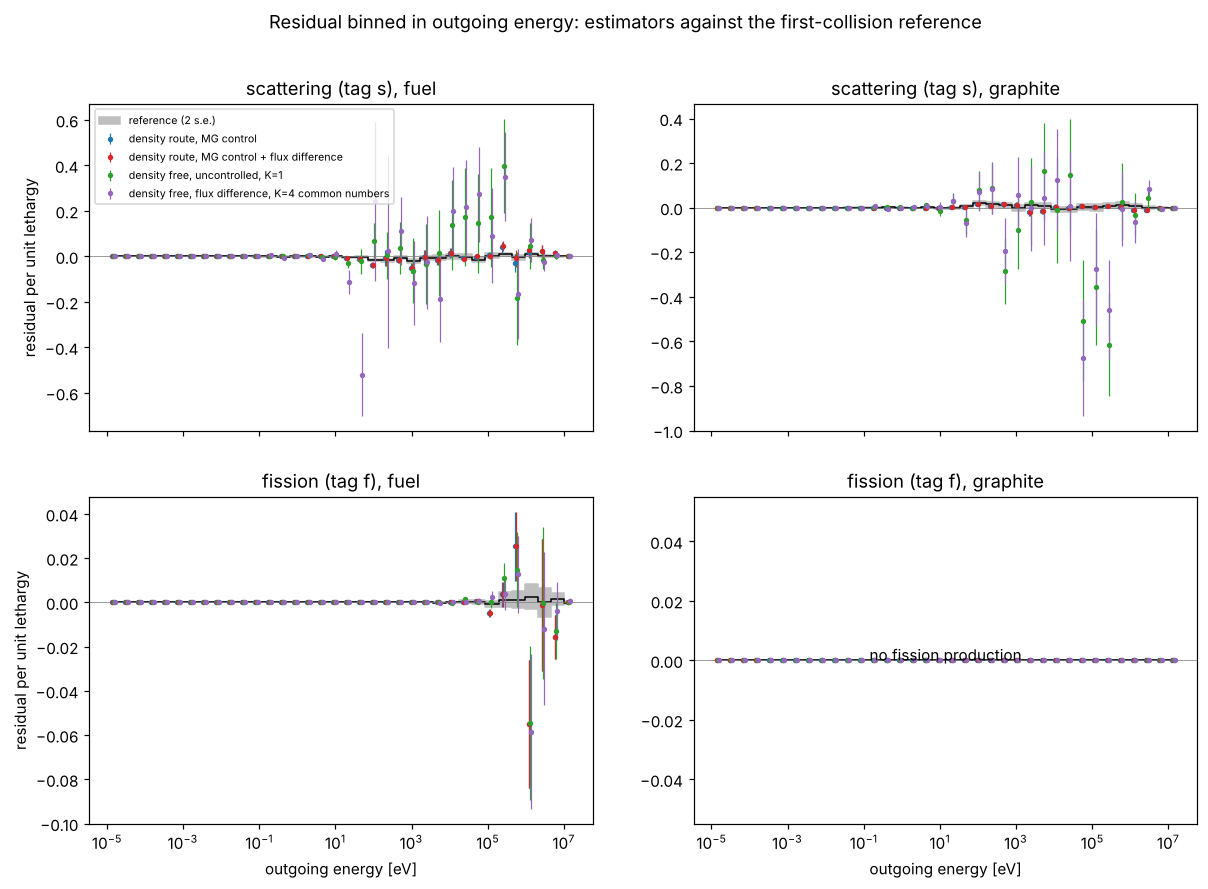
\includegraphics[width=\textwidth]{figures/controlled_energy.png}
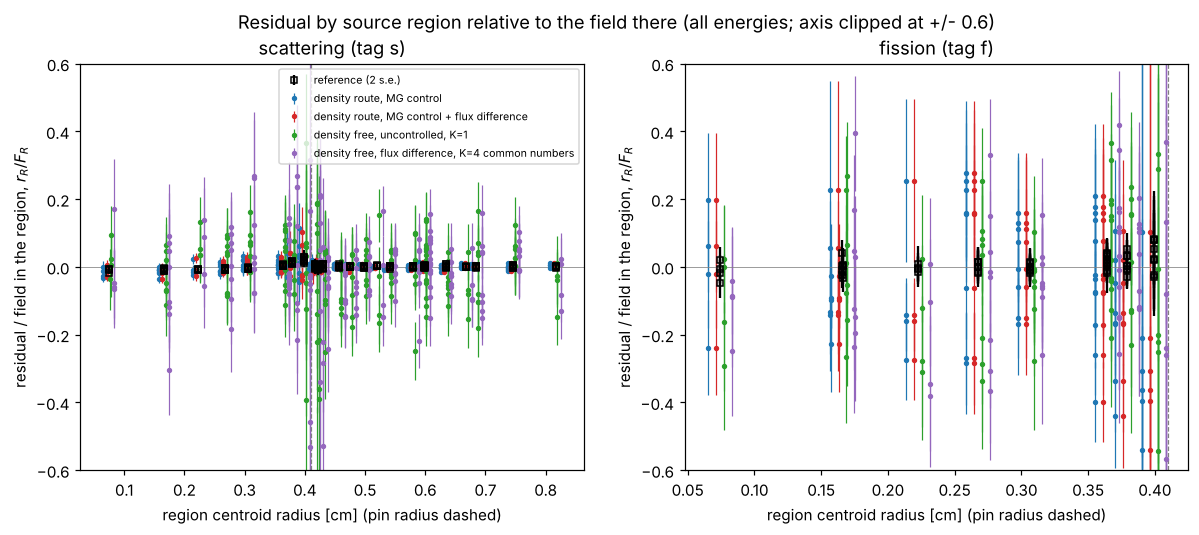
\includegraphics[width=\textwidth]{figures/controlled_space.png}
\caption{Top: residual per unit lethargy. Bottom: residual by region relative to the field there, against
the region's centroid radius.}\label{fig:res:energy}
\end{figure}

\textbf{Energy} (Figure~\ref{fig:res:energy}, top). In the fuel the scattering residual is negative
just below 4 eV and changes sign through the resonance group: the 8-group field spreads emission
uniformly in lethargy within a group as weighted by an infinite-medium-like spectrum, while the true
emission in the pin dips at every U-238 resonance (fewer neutrons there to scatter) and rises
between them. The fission residual lives between 100 keV and 10 MeV, where it reflects the difference
between the CE fission spectrum of the actual incident spectrum and the one group-collapsed $\chi$
of the MG data.

\textbf{Space} (Figure~\ref{fig:res:energy}, bottom). The reference residual is within $\pm3$\% of the
field everywhere except the small regions cut by the pin surface, where it reaches $\pm15$\%: the
field is flat within a region while the true emission has a gradient across the fuel--moderator
interface. The density route resolves these; the density-free estimators do not at this sample
size.

\begin{figure}[t]\centering
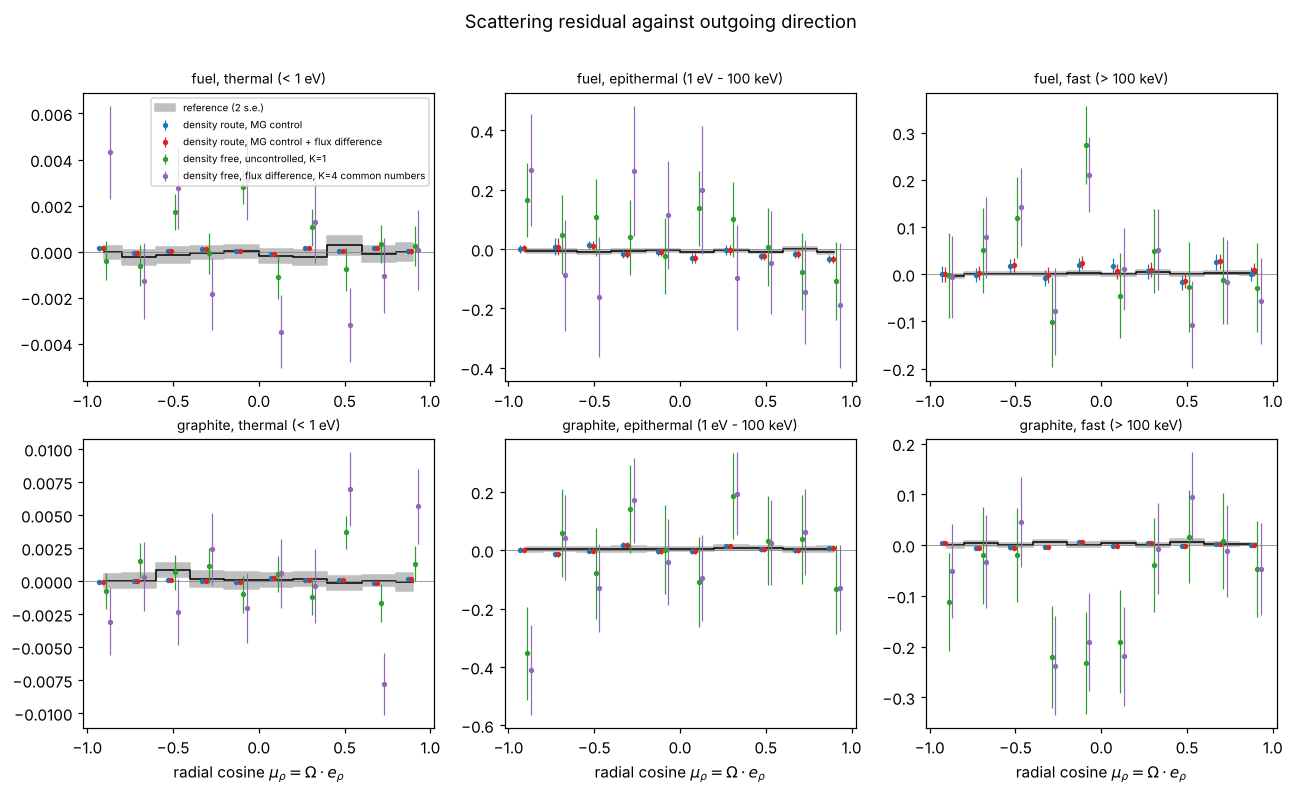
\includegraphics[width=\textwidth]{figures/controlled_angle.png}
\caption{Scattering residual against the radial cosine of the outgoing direction.}\label{fig:res:angle}
\end{figure}

\textbf{Angle} (Figure~\ref{fig:res:angle}). The field is isotropic; any angular residual comes from the
anisotropy of real scattering (forward-peaked in the lab, especially in graphite at MeV energies) and
of the flux near the pin surface. At this resolution the reference resolves no angular structure, so
this binning tests the estimators' directional noise.

\subsection{Where the variance comes from}

\begin{figure}[t]\centering
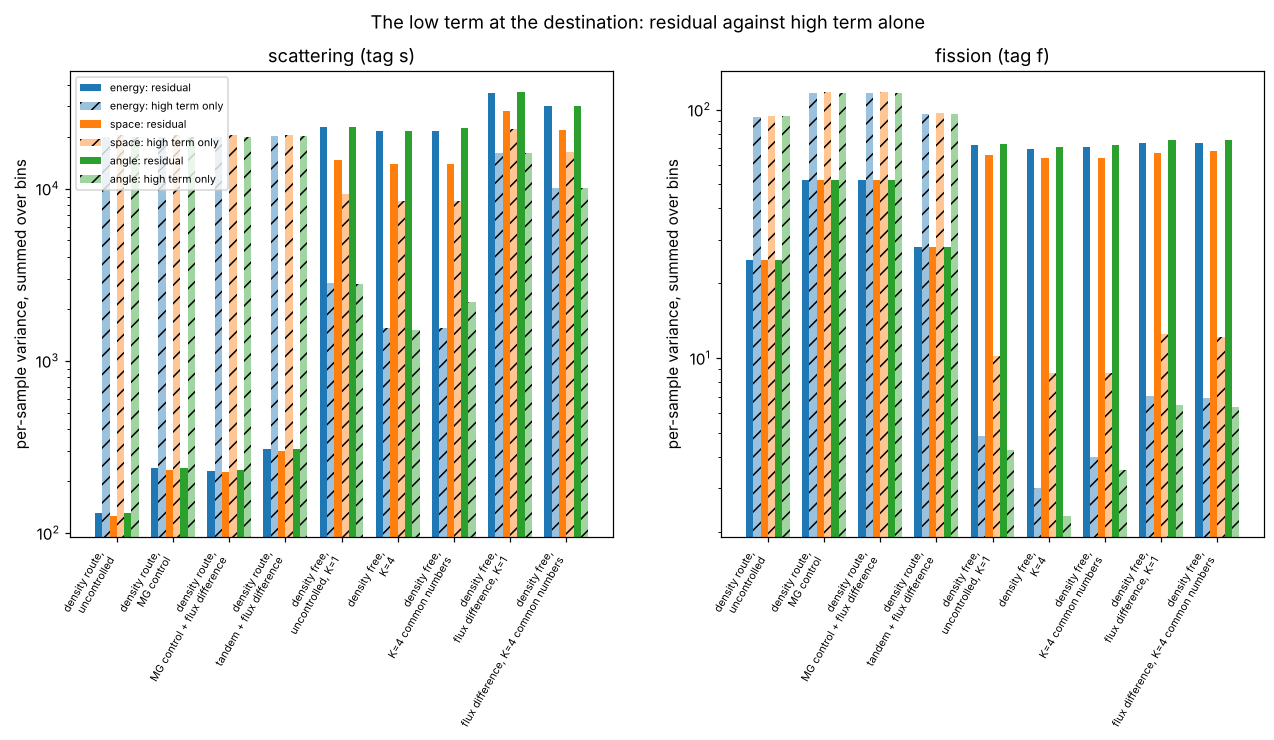
\includegraphics[width=\textwidth]{figures/controlled_low_term.png}
\caption{Per-sample variance of the residual (solid) and of the high term alone (hatched), per
binning.}\label{fig:res:lowterm}
\end{figure}

\begin{table}[t]\centering\small
\begin{tabular}{lrrrr}
\toprule
Variant & $s$: residual & $s$: high only & $f$: residual & $f$: high only\\
\midrule
density route, uncontrolled & \textbf{130} & 19{,}900 & \textbf{24.7} & 93.7\\
density route, MG control & 238 & 20{,}000 & 52.1 & 117\\
density route, tandem + flux difference & 308 & 20{,}100 & 27.9 & 95.8\\
density free, uncontrolled, $K=1$ & 22{,}800 & 2{,}840 & 72.0 & 4.86\\
density free, $K=4$ & 21{,}500 & 1{,}560 & 69.7 & 3.00\\
density free, flux difference, $K=1$ & 35{,}900 & 16{,}000 & 73.7 & 7.07\\
density free, flux difference, $K=4$ c.n. & 30{,}100 & 10{,}100 & 73.6 & 6.92\\
\bottomrule
\end{tabular}
\caption{Per-sample variance summed over the 72 energy bins.}\label{tab:res:var}
\end{table}

Three findings (Figure~\ref{fig:res:lowterm}, Table~\ref{tab:res:var}):
\begin{enumerate}
\item \textbf{Pointwise cancellation is the density route's whole advantage.} Its high term alone is
  the noisiest of all ($2\times10^4$ for scattering): the elastic image densities are large when the
  image falls on a resonance or the laboratory Jacobian is large. At the destination's state the low
  term removes 99.3\% of it.
\item \textbf{The density-free residual is dominated by the low term}: $2.05\times10^4$ of the
  scattering variance and 69 of the fission variance are the field's own integral estimated by Monte
  Carlo.
\item \textbf{The sampled high term is good}: 7 (scattering) to 19 (fission) times quieter than the
  evaluators' at $K=1$, 33 to 56 times at $K=16$.
\end{enumerate}

\begin{figure}[t]\centering
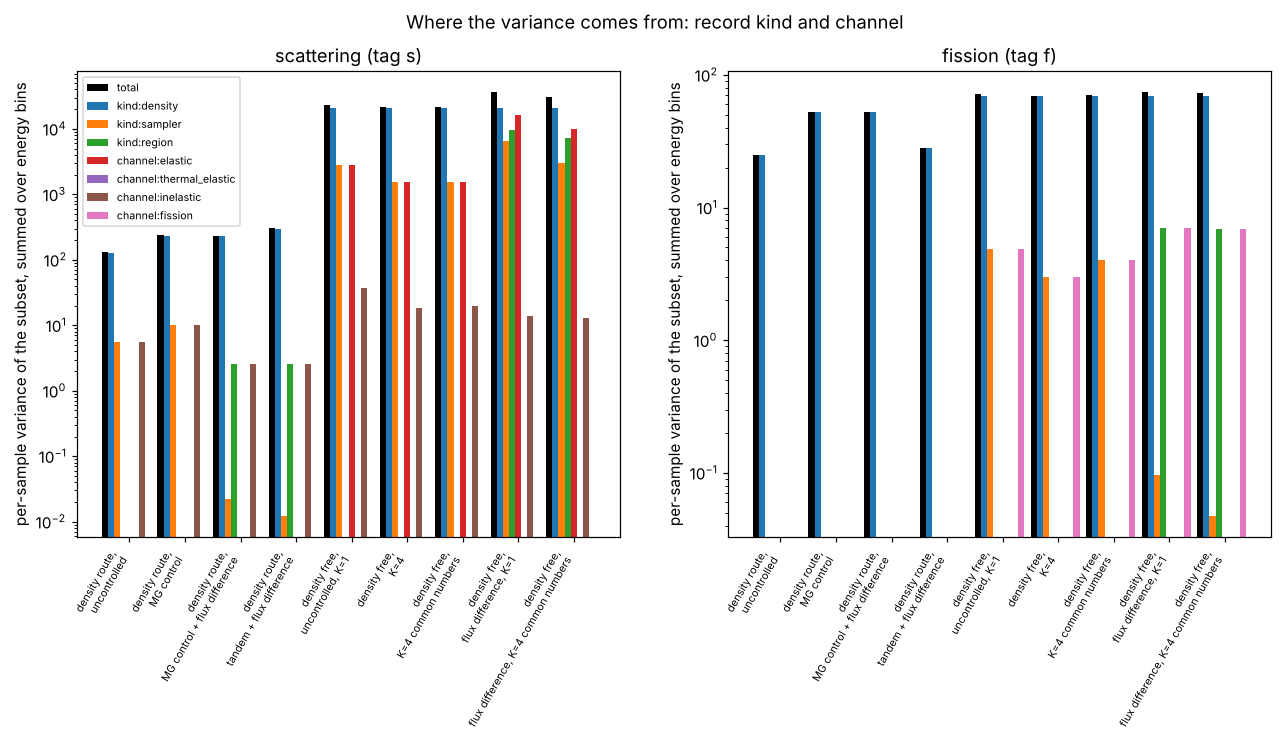
\includegraphics[width=\textwidth]{figures/controlled_decomposition.png}
\caption{Variance of the records of each kind (density branch, sampler particles on a path, region-term
particles) and channel. In every density-free variant the density branch, which then carries only the
low term, dominates; among scattering channels elastic carries almost all of the sampled variance.}\label{fig:res:decomp}
\end{figure}

\begin{figure}[t]\centering
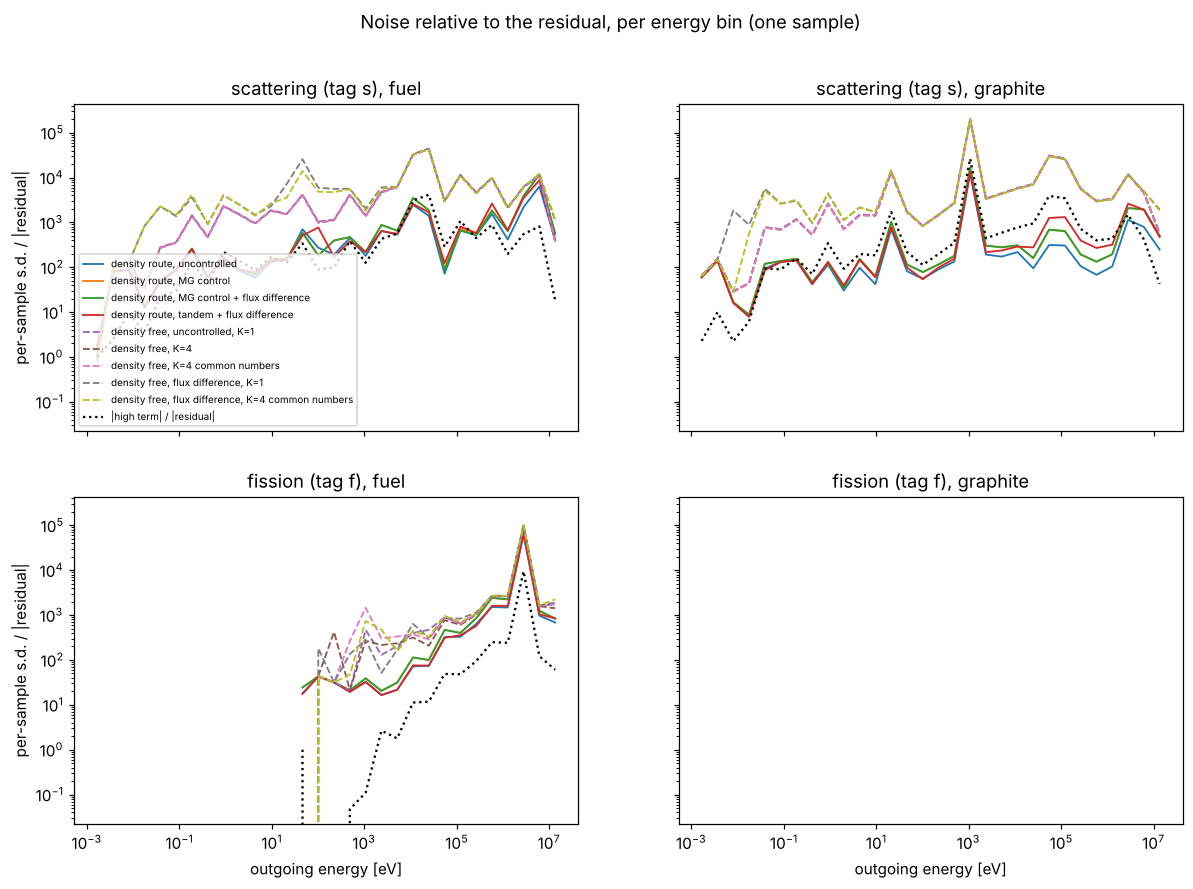
\includegraphics[width=\textwidth]{figures/controlled_relative_noise.png}
\caption{Per-sample standard deviation over $|r|$ per energy bin. The dotted line is the ratio of the
production to the residual: an estimator with production-scale noise sits on or above it. The density
route sits a factor of 3--30 below it, the density-free route on it.}\label{fig:res:relnoise}
\end{figure}

\subsection{Parameters}

\begin{figure}[t]\centering
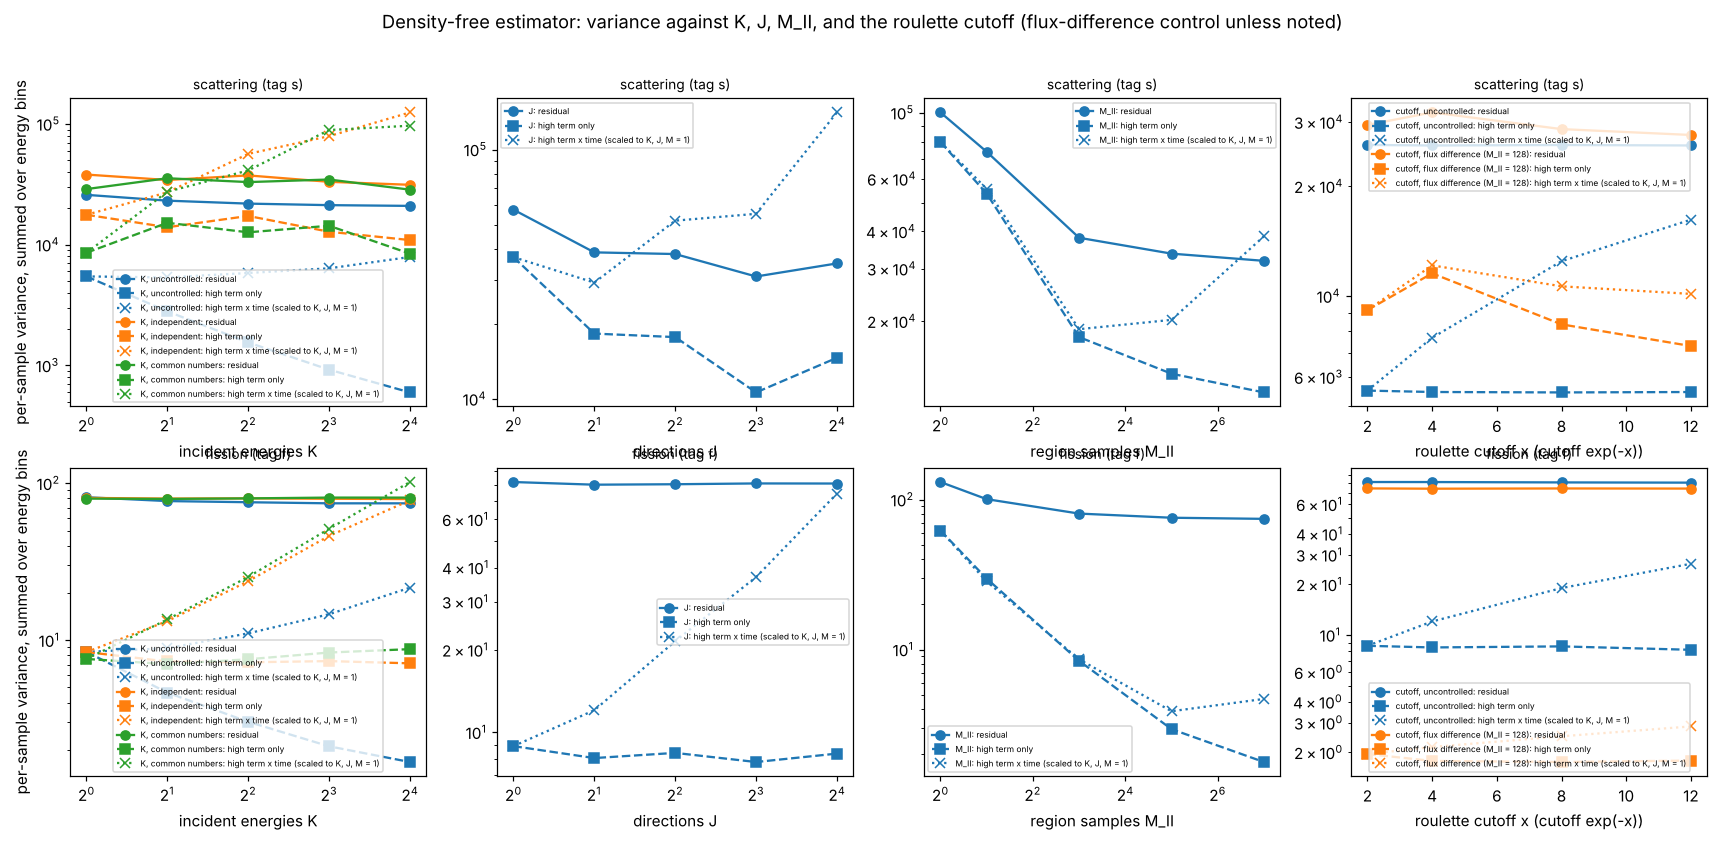
\includegraphics[width=\textwidth]{figures/controlled_scans.png}
\caption{Density-free scans: variance of the residual (circles) and of the high term alone (squares)
against $K$, $J$, $M_{II}$ and the roulette cutoff; crosses: high term $\times$ time.}\label{fig:res:scans}
\end{figure}

Figure~\ref{fig:res:scans}: more incident energies help roughly as $K^{-0.8}$, but each costs a
collision sample, so variance $\times$ time is flat; more directions help with diminishing returns;
the region term of the flux-difference control falls as $1/M_{II}$ to a floor set by term I; the
roulette cutoff hardly matters. For fission the flux-difference control works (high-term variance 1.8
at $M_{II}=128$ against 8.4 uncontrolled): the fission spectrum barely depends on $E'$, so the region's
isotropic MG flux captures the incident integral. For scattering it hurts: the isotropic,
region-averaged lifted flux is a poor match to $\psi(E')$ on a path through the pin's resonances.

\subsection{Does the noise scale with the residual?}

\begin{figure}[t]\centering
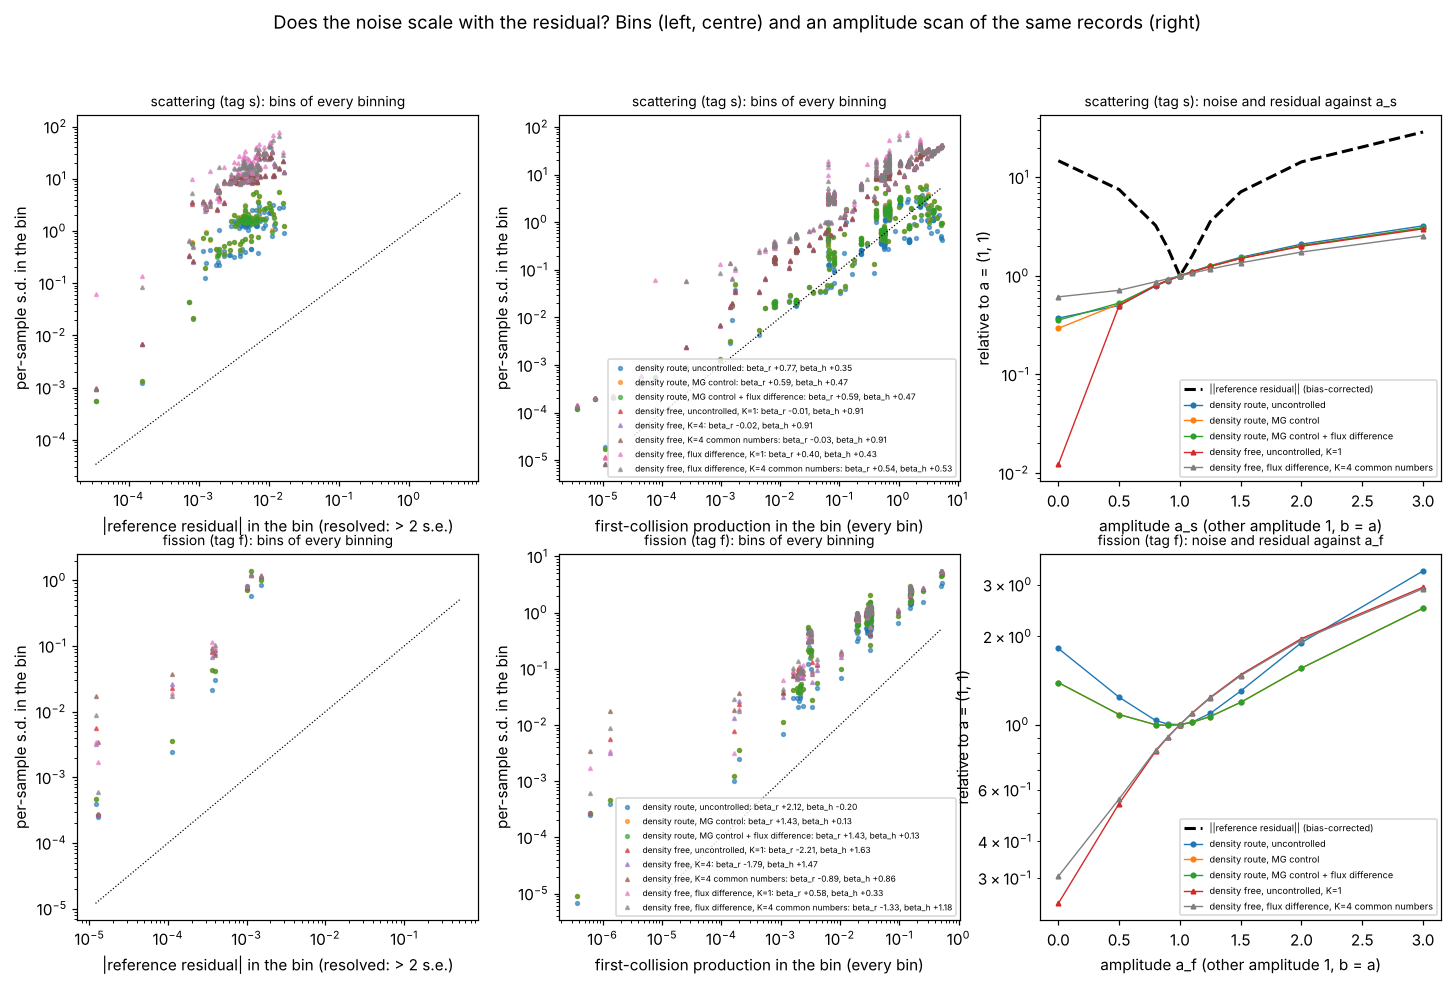
\includegraphics[width=\textwidth]{figures/controlled_noise_scaling.png}
\caption{Left, centre: per-sample standard deviation per bin against the reference residual and the
production. Right: the same records reweighted for other amplitudes, where the residual's norm grows
10 to 400 times.}\label{fig:res:scaling}
\end{figure}

Fitting $\log\sigma=\alpha+\beta_r\log|r|+\beta_h\log h$ over resolved scattering bins, the density
route has $\beta_r\approx0.5$--$0.8$ through its pointwise cancellation while every uncontrolled
density-free variant has $\beta_r\approx0$, $\beta_h\approx0.9$: production-scale noise. The amplitude
scan (Figure~\ref{fig:res:scaling}, right) asks the sharper question: when the residual grows 10 to
400 times, the noise of every estimator changes by at most 3 times, in proportion to the high term.
At the converged field no member of the family has noise that falls with the residual; what remains
is the integration noise of the high term over $\vO'$ and $E'$.

\begin{figure}[t]\centering
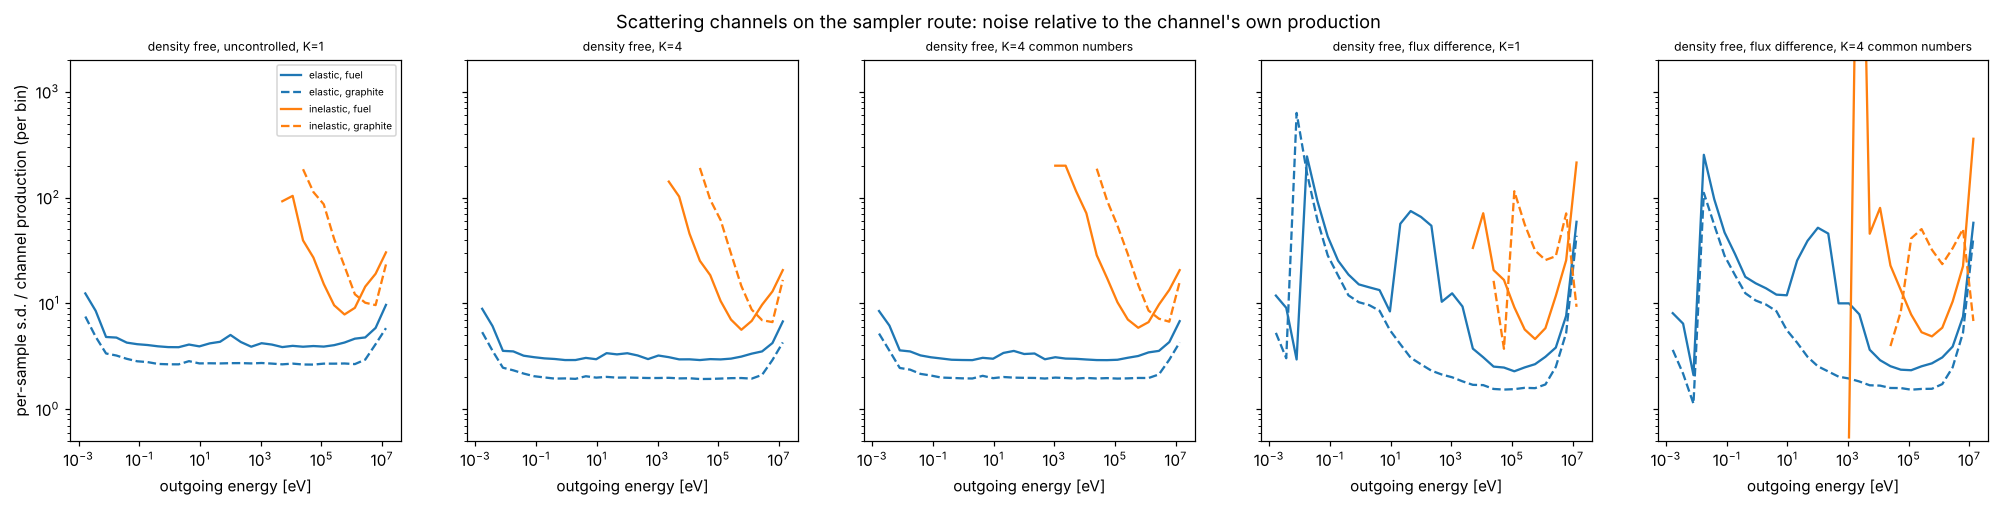
\includegraphics[width=\textwidth]{figures/controlled_channels.png}
\caption{Per-channel noise relative to the channel's own production on the sampler route: elastic about
3--4 per sample per bin, inelastic 10--100 (its production is small and sharply thresholded). The
flux-difference control lowers the elastic noise above 100 keV, where the flux is nearly isotropic and
smooth, and raises it in the resonance range.}\label{fig:res:channels}
\end{figure}

\begin{figure}[t]\centering
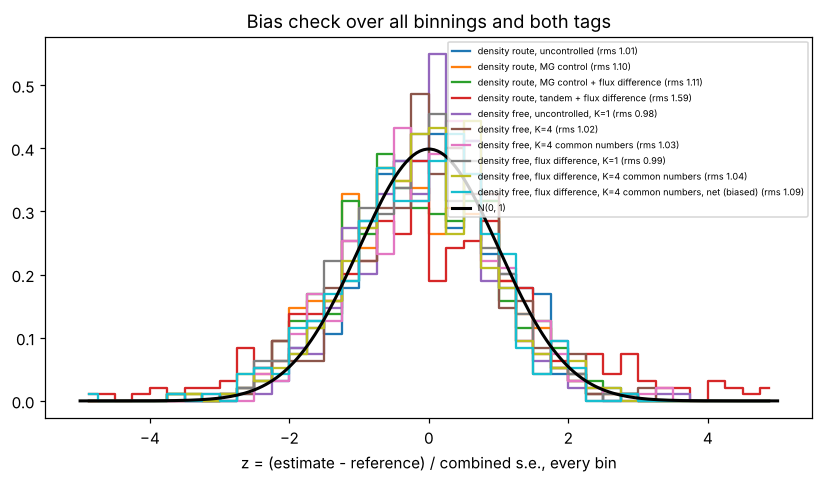
\includegraphics[width=0.85\textwidth]{figures/controlled_z.png}
\caption{Bias check: standardized differences from the reference over every resolved bin of the three
binnings and both tags. Unbiased variants follow the normal density; the net assignment (biased by
construction) is wider.}\label{fig:res:z}
\end{figure}

\subsection{The low term made exact}

With the low term exact (in a tally, or in netting bins), the efficiency (variance $\times$ time,
energy binning) is: scattering, density route 90 against 680--880 density-free; fission, density route
2.0 against 0.19--0.36 density-free. Each route should be used for what it is good at: the density
route for channels with an evaluator and pointwise cancellation, the sampler route with an exact low
term for fission and for channels without densities.

\section{The first end-to-end measurement}\label{sec:res:stage8}

% Stage 8: the first end-to-end measurement. Numbers from
% examples/rmc/stage8_analysis.py on the runs in examples/rmc/results/stage8.

\newcommand{\refk}{0.64202}
\newcommand{\refksd}{0.00049}
\newcommand{\refT}{151}


This section reports the first run of the whole method: the MG field, the residual for both tags, the
cancellers of Section~\ref{sec:cancellation}, the flights, and the correction tally. All of it ran
together on the graphite pincell and was compared with OpenMC's continuous-energy eigenvalue
calculation of the same model. The question is whether the method works at all: whether it is
unbiased, how its variance per particle and per second compares with analog Monte Carlo, and what
engineering could recover. It is not yet the question of whether it wins.

\subsection{Setup}

\paragraph{Problem.} The graphite-moderated UO$_2$ pincell of Section~\ref{sec:res:setup} has fuel
pin, gap and graphite block, reflective on every face, at 294~K with ENDF/B-VIII.0 data. Its
infinite-lattice multiplication factor is $k\approx0.642$. It is far from critical because the
moderator-to-fuel ratio is far from optimal: thermal absorption in the large graphite block competes
with the fuel.

The spectrum is strongly thermal. Fission neutrons born near 2~MeV need about 115 collisions with
carbon ($\xi\approx0.158$) to reach thermal energies. Most of those collisions happen in the
graphite, far from the pin, so the slowing-down source near the fuel is close to the
$1/E$ asymptotic form, apart from the dips at the $^{238}$U resonances. This has two consequences.
\begin{itemize}
\item Most fissions are induced by thermal neutrons that entered the pin from the moderator. The
  fission source is peaked at the pin surface and depressed at its centre: the thermal flux dips
  inside the absorbing pin.
\item The scattering ratio $c$ is close to one almost everywhere. That makes the emission-source
  iteration of Section~\ref{sec:convergence} slow and its generations strongly correlated.
\end{itemize}

\paragraph{Field.} The MG field is the 8-group flat-source random-ray solution, with prescribed
(exact) region volumes. It has 172 regions: the cells cut by the $12\times12$ source-region mesh. Of
these, 60 are fuel regions. The field eigenvalue is $k_{MG}=0.64257$, already within $55$~pcm of
the CE reference. The MG answer is close, and the correction only has to supply the fine-energy and
angular structure that 8 groups cannot represent.

\paragraph{Reference.} OpenMC eigenvalue runs, single-threaded:
\begin{itemize}
\item 4 independent replicas;
\item each with $2\times10^4$ particles per batch, 20 inactive and 50 active batches ($10^6$ active histories);
\item fission and $\nu$-fission tallied on the same fuel regions.
\end{itemize}
The results:
\begin{itemize}
\item $k=\refk\pm\refksd$ (the spread of the replicas; each replica's own batch estimate is $0.00058$);
\item $\refT$~s of active time per replica.
\end{itemize}

\paragraph{RMC runs.} \code{examples/rmc/stage8.py} runs each variant in 3 independent replicas. Two
campaigns were run:
\begin{itemize}
\item \textbf{First campaign.} 5 inactive and 30 active generations, $N_s=N_f=2000$ residual samples,
  a bank resampled to $N_\delta=2\times10^4$, $N_B=2\times10^4$ netting particles, and a CE
  correction tally with $2\times10^4$ backward points per generation.
\item \textbf{Tuned campaign} (combined variants only). 40 inactive and 60 active generations,
  $N_\delta=2\times10^5$, $N_B=4\times10^4$, and a correction tally with $10^4$ points plus the MG
  control (a one-off low tally of $4\times10^5$ points, Section~\ref{sec:tallies}). This campaign
  tallies $\nu$-fission.
\end{itemize}
Every replica is single-threaded. The figures of merit use active time only, on both sides.

\paragraph{Variants.} These are the classes of Section~\ref{sec:cancellation}:
\begin{center}\small
\begin{tabular}{@{}lll@{}}
\toprule
variant & residual routes & cancellation \\
\midrule
none & density route, both tags & none \\
binned netting & density route, both tags & netting (zones $3\times3$ per material, group bins) \\
binned, exact low (f) & s density, f sampler & netting, fission low term in closed form per bin\\
exact only & s density, f sampler & destination pooling + regional point kernel \\
exact + binned netting & s density, f sampler & pooling + regional + netting \\
exact + finer netting & as above & netting with $12\times12$ zones and 4 sub-bins per group \\
\bottomrule
\end{tabular}
\end{center}

\subsection{Stability: the absolute weight of the bank}

\begin{figure}[t]\centering
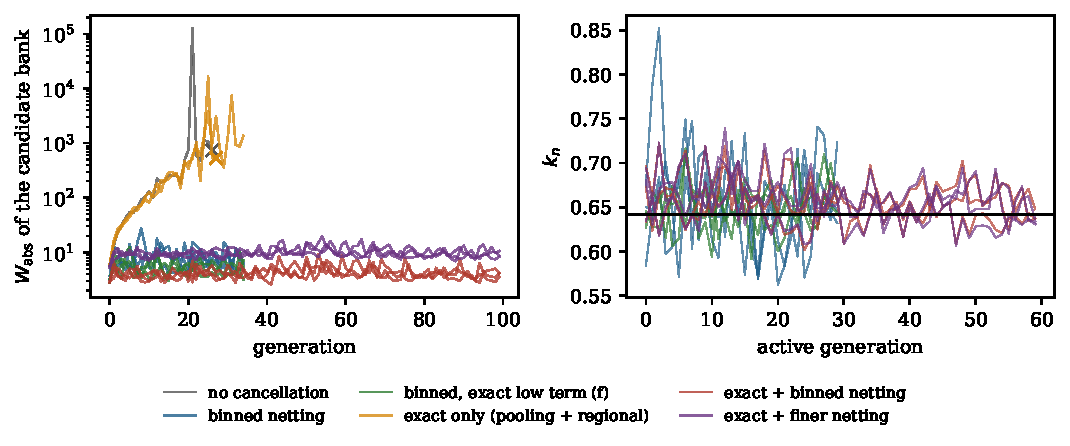
\includegraphics[width=\textwidth]{figures/stage8_wabs_k.pdf}
\caption{Left: absolute weight $\Wabs$ of the candidate bank (after cancellation) against generation,
for every variant and replica. A cross marks an estimator failure: the fission production $f$ turned
negative and the eigenvalue update became undefined. Right: the generation estimate $k_n$ over the
active generations of the variants that ran to completion, against the CE reference (black line).}
\label{fig:s8:wabs}
\end{figure}

Figure~\ref{fig:s8:wabs} answers the first question: without cancellation the method does not run.
\begin{itemize}
\item \textbf{No cancellation.} $\Wabs$ grows geometrically, by about $30\%$ per generation. Generation
  27 fails with $\Wabs\approx735$: the signed bank's noise exceeded the production it corrects and
  $f<0$. This is the instability of Section~\ref{sec:wabs}: with $\kappa\eta>1$ no stationary $\Wabs$
  exists.
\item \textbf{Exact methods alone.} Destination pooling and the regional kernel do not stop the
  growth. Pooling cancels the fission residual very well: $\Wabs$ of the fission records falls from
  $2.8$ to $0.75$ per generation. But scattering carries most of the absolute weight, and only
  netting touches it. One replica failed at generation 28, the other reached $\Wabs\approx1360$.
\item \textbf{Netting.} Every variant with netting is stable, with $\Wabs$ between 4 and 10:
  \begin{itemize}
  \item the coarse representation ($3\times3$ zones) holds $\Wabs\approx4$--$8$;
  \item adding the exact fission methods lowers it to $\approx4.4$;
  \item the finer representation, counter-intuitively, raises it to $\approx10$. More bins means
    fewer particles of opposite sign per bin, so there is less to cancel. This is the trade-off of
    Section~\ref{sec:netting-bias}: a finer representation has less bias but cancels less.
  \end{itemize}
\end{itemize}
In the tuned combined run, one typical generation looks like this:
\begin{itemize}
\item netting reduces $\Wabs$ from $11.2$ to $4.8$ over 645 occupied bins;
\item pooling moves $\approx700$ fission records into the pools and cuts their absolute weight by a
  factor $3.8$;
\item the regional kernel is eligible for only $\approx20$ of $\approx1300$ fission children.
\end{itemize}
The regional kernel acts so rarely because fission children come almost entirely from tag-s parents.
These are thermal neutrons arriving from the graphite, not the tag-f parents near the pin that the
kernel requires. In this problem it is inert, and its cost buys nothing.

\begin{figure}[t]\centering
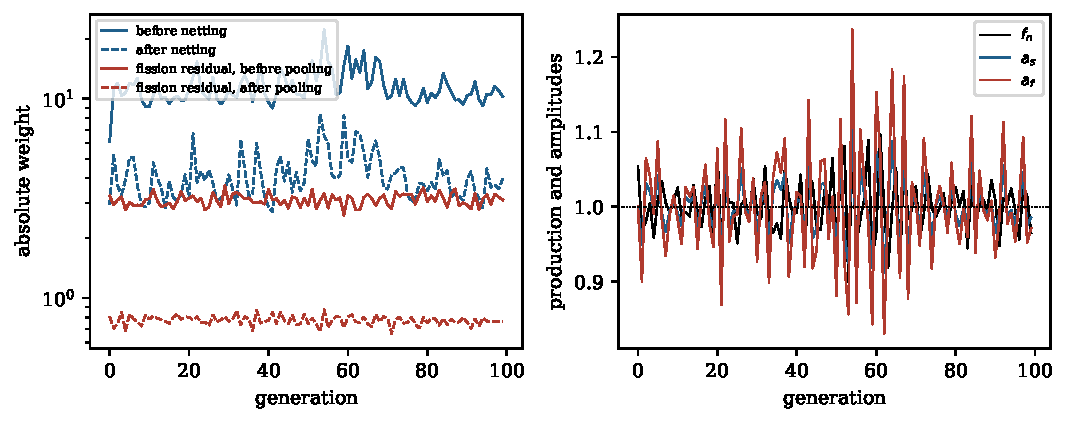
\includegraphics[width=\textwidth]{figures/stage8_diagnostics.pdf}
\caption{One replica of the tuned combined variant, generation by generation. Left: absolute weight
before and after netting (whole candidate bank), and of the fission residual before and after
destination pooling. Right: the production $f_n$ and the amplitudes $a_s$, $a_f$. Netting removes
about half of the bank's absolute weight every generation; pooling removes three quarters of the
fission residual's. The production fluctuates by about 4\% and the fission amplitude by about 8\%:
this noise, fed back through the iteration, is the leading candidate for the eigenvalue bias.}
\label{fig:s8:diag}
\end{figure}

Figure~\ref{fig:s8:diag} shows the stationary state. What remains after netting is about four times
the absolute weight of the fission residual after pooling. The scattering residual and its children,
which only netting touches, carry the variance.

\subsection{Bias}

\begin{table}[t]\centering\small
\caption{End-to-end results against the CE reference ($k=\refk$). The columns are:
$\Delta k$, the bias in pcm; $z_{bm}$ and $z_{rep}$, the bias in units of its standard error from
5-generation batch means and from the spread of the 3 replicas; $\overline{\Wabs}$, over active
generations; $T$, the active time per replica in seconds; the $k$ figure-of-merit ratio
(RMC/reference) with each error estimate; the fuel-region shape FOM ratio; and the projected
speedup $s$ of Section~\ref{sec:s8:projection}. The first two rows are the first campaign (30 active
generations, $N_\delta=2\times10^4$); the last two are the tuned campaign (60 active,
$N_\delta=2\times10^5$, MG-controlled $\nu$-fission tally).}\label{tab:s8}
\setlength{\tabcolsep}{3.5pt}
\resizebox{\textwidth}{!}{%
\begin{tabular}{@{}lrrrrrrrrrr@{}}
\toprule
variant & $k$ & $\Delta k$ & $z_{bm}$ & $z_{rep}$ & $\overline{\Wabs}$ & $T$ &
FOM$_k$ (bm) & FOM$_k$ (rep) & FOM$_{shape}$ & $s$\\
\midrule
\csname @@input\endcsname figures/stage8_table.tex
\bottomrule
\end{tabular}}
\end{table}

\paragraph{The eigenvalue is biased high.} Every completed variant overestimates $k$, by
$860$--$1450$~pcm (Table~\ref{tab:s8}). Taken one at a time, the replica-based significance is
modest, between $1.4\sigma$ and $3.3\sigma$.

The four variants agree in sign and size, but that is weaker evidence than it looks. Every variant
used the same three seeds. The residual's random numbers depend only on the seed, the generation
and the sample index, so the variants share their residual samples replica by replica. The replica
with seed 2001 is low in every variant, and the others are high in every variant. The variants
are therefore three paired samples, not twelve independent ones.

Section~\ref{sec:res:followup} repeats the baseline with six new seeds and scans $N$. There, a
positive bias of $+1050\pm360$~pcm survives at $N=2000$.

That section also takes back an argument made here first. This section originally dismissed the
netting bias because the bias barely moved between the coarse and fine representations. But both
representations bin by group or quarter-group, which is far wider than a resonance, so neither
resolves the within-group structure that netting's bias depends on. The deterministic netting bias
of Section~\ref{sec:iteration} and the noise-driven normalization bias are tested directly in
Section~\ref{sec:res:followup}.

\paragraph{Batch means underestimate the error.} The replica spread of $k$ is $2$--$3$ times the
batch-means estimate. Within a replica, the estimated autocorrelation time is only $\tau\approx2$--$5$
generations. The long excursions of Figure~\ref{fig:s8:wabs} explain the gap: they are the slow
scattering modes, with $\tau\sim(1+c)/(1-c)\sim10^2$. A lag-window estimate over 60 generations
cannot see them. So the honest error is the replica one, and the $z_{bm}$ column overstates
significance. The nine independent replicas of Section~\ref{sec:res:followup} give $\tau=21$
collision generations. That is about half of a neutron lifetime (37 collisions), so the correlation is
long only in units of collision generations.

\begin{figure}[t]\centering
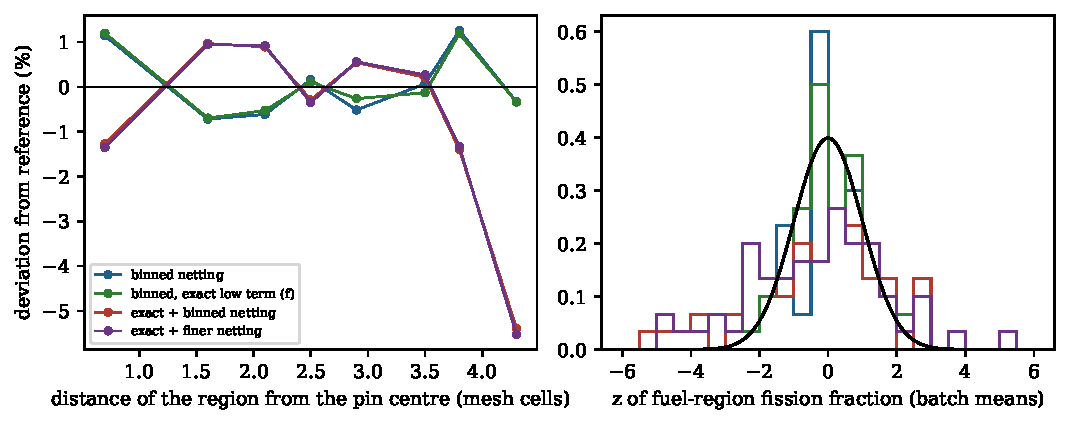
\includegraphics[width=\textwidth]{figures/stage8_shape.pdf}
\caption{Fission (or $\nu$-fission) rate by fuel region, normalized to unit sum. Left: mean relative
deviation from the reference against the region's distance from the pin centre. Right: histogram of
standardized differences (batch-means errors), against the standard normal density.}
\label{fig:s8:shape}
\end{figure}

\paragraph{The fission-rate shape.} With the CE correction tally (the first campaign), the fuel-region
shape agrees with the reference: $\chi^2=66$ for 60 regions, and no radial trend
(Figure~\ref{fig:s8:shape}). The $\pm1\%$ pattern that both binned variants share is the reference's
own noise, which both comparisons inherit.

The MG-controlled tally of the tuned campaign shows a $-5\%$ deficit in the outermost fuel regions,
and $\chi^2\approx255$. The pattern is the same for the coarse and fine netting, which share nothing
except the one-off MG low tally. That points to the low tally: its $4\times10^5$ backward points are
drawn once with a fixed seed and reused in every generation. Their sampling error is therefore
\emph{frozen}: it acts as a bias of the run rather than averaging away. It is largest in the small
partial regions cut by the pin surface, which receive the fewest uniform points.

This is a design error, not a property of the estimator. The low term of the MG control is the MG
reaction rate $V_R\sum_g\nu\Sigma_{f,g}\phi_{R,g}$, known in closed form from the field. It should be
computed that way, or at least redrawn every generation.

\subsection{Variance per particle and figure of merit}

\paragraph{Per particle.} The variance of $k$ per unit of work compares as follows:
\begin{itemize}
\item \textbf{RMC, tuned combined variant.} A generation processes $4\times10^3$ residual samples
  and $4\times10^4$ flights. The per-generation $k_n$ scatters by $0.021$, so the variance per
  particle-generation is $0.021^2\times4.4\times10^4\approx19$.
\item \textbf{Reference.} The batch-to-batch scatter of $k$ is $0.0041$ at $2\times10^4$ histories, so
  the variance per history is $0.34$.
\end{itemize}
Measured per particle and ignoring correlation, the method is $\approx60$ times worse. Counting the
correlation between generations, as the replica spread does (on both sides), it is $\approx1500$
times worse.

The per-particle variance is large because the residual estimate's absolute weight is large. In
the tuned run each generation's candidate bank holds about 12 units of absolute weight per unit of
fission production, before netting:
\begin{itemize}
\item $6.7$ from the scattering residual records;
\item $0.8$ from the fission residual after pooling ($3.1$ before);
\item $4.4$ from the children of the previous bank.
\end{itemize}
Netting keeps about $37\%$. The flights and netting only carry and contract what the residual
injects, so the residual estimator is the noise source. Its noise is not residual-scale: per sample
it is the integration noise of the high term over $\mathbf\Omega'$ and $E'$
(Section~\ref{sec:res:controlled}). Part of the scattering residual's signed mass is, in addition,
the amplitude term of Section~\ref{sec:iteration} (Section~\ref{sec:res:followup}).

\paragraph{Per second.} The figure of merit $1/(\sigma^2T)$ of $k$ for the tuned combined variant,
relative to the reference, is:
\begin{center}
\begin{tabular}{@{}lcc@{}}
\toprule
 & batch-means $\sigma$ & replica $\sigma$\\
\midrule
measured & $0.020$ & $0.0015$\\
projected (Section~\ref{sec:s8:projection}) & $0.068$ & $0.0049$\\
\bottomrule
\end{tabular}
\end{center}
The batch-means figure is optimistic and the replica figure, from only three replicas, is uncertain
by about a factor of two. The truth is nearer the replica figure.

The best measured $k$ figure of merit belongs to the low term in closed form (binned, exact low):
$0.043$ with batch means. It also has the smallest bias.

The shape figure of merit, the mean relative variance over the 60 fuel regions, is $10^{-3}$ of the
reference for every variant. The correction tally is dominated by its backward points and the bank's
collision estimator, and both carry the bank's full absolute weight into every region.

\subsection{Follow-up: the bias, the amplitudes, and history-based flights}\label{sec:res:followup}

The first measurement left three questions:
\begin{itemize}
\item whether the bias is the normalization bias of a noisy iteration or netting's deterministic bias;
\item where the noise comes from;
\item whether history-based flights, which make a generation fission-to-fission, shorten the
  correlation enough to pay for themselves.
\end{itemize}
Every run below is the tuned combined variant (40 inactive and 60 active generations, $N_\delta=2\times10^5$,
$N_B=4\times10^4$) unless stated otherwise. The runs are in
\code{results/stage8\_followup} under \code{examples/rmc}, and \code{stage8\_followup\_analysis.py}
analyses them.

\begin{table}[t]\centering\small
\caption{Follow-up runs. Columns: $n$, the number of replicas; $\Delta k$, the bias against the
reference with its standard error; paired, the difference from the baseline replica with the same
seed (same residual samples); $\overline{\Wabs}$, the bank's mean absolute weight; $\sigma_{gen}$, the
per-generation spread of $k_n$; $T$, the active time per replica in seconds; FOM$_k$, the figure of
merit relative to the reference. The errors of a replica mean use $\sigma_{gen}\sqrt{\tau/n_{gen}}$
with $\tau=21$ generations, measured from the nine independent baseline replicas; the first row uses
their spread directly.}
\label{tab:fu}
\setlength{\tabcolsep}{3.5pt}
\resizebox{\textwidth}{!}{%
\begin{tabular}{@{}lrrrrrrr@{}}
\toprule
run & $n$ & $\Delta k$ (pcm) & paired (pcm) & $\overline{\Wabs}$ & $\sigma_{gen}$ & $T$ & FOM$_k$\\
\midrule
\csname @@input\endcsname figures/followup_table.tex
\bottomrule
\end{tabular}}
\end{table}

\begin{figure}[t]\centering
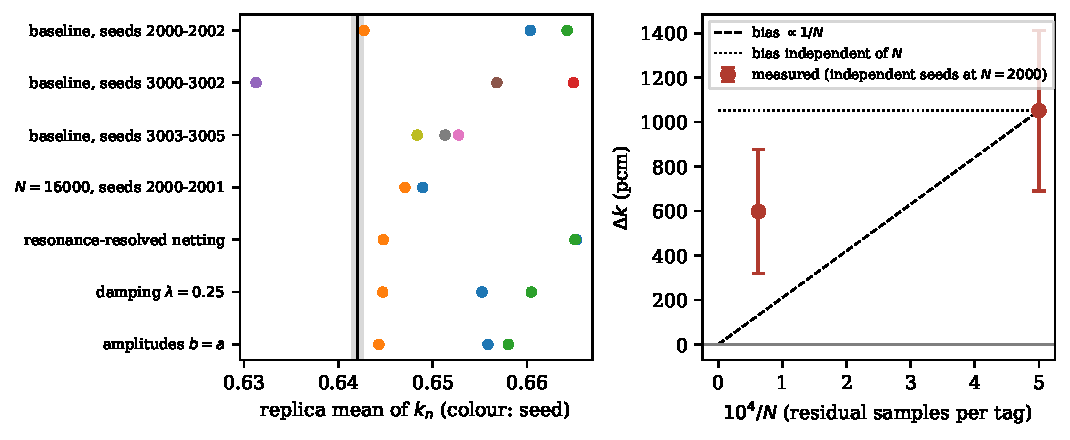
\includegraphics[width=\textwidth]{figures/followup_bias.pdf}
\caption{Left: replica means of $k_n$ for every run, coloured by seed. Replicas with the same seed
share their residual samples, which is why the seed-2001 replica (orange) is low in every run of the
first group. The vertical line and band are the reference and its replica spread. Right: the bias
against $1/N$, with the two simple models.}\label{fig:fu:bias}
\end{figure}

\paragraph{Independent seeds.} Six new replicas (seeds 3000--3005) give $k$ between $0.631$ and
$0.665$. With the original three, the nine independent baseline replicas give:
\begin{itemize}
\item $\Delta k=+1050\pm360$~pcm, a positive bias at $2.9\sigma$; eight of the nine replicas lie above
  the reference;
\item a replica spread of $0.0108$ against a per-generation spread of $0.018$ over 60 generations,
  which means an integrated autocorrelation time of $\tau=21$ collision generations.
\end{itemize}

\paragraph{The bias against $N$.} With $N=16000$ residual samples per tag (seeds 2000 and 2001):
\begin{itemize}
\item the per-generation spread falls from $0.021$ to $0.0066$, a factor of $3.2$, close to $\sqrt8$;
\item the bank's absolute weight falls from $4.4$ to $1.8$, because more samples per bin cancel
  better;
\item the bias is $+600\pm280$~pcm.
\end{itemize}
A bias proportional to $1/N$ would be $130$~pcm here; one independent of $N$ would stay at $1050$.
The measurement lies between the two and is $1.7\sigma$ from each (Figure~\ref{fig:fu:bias}). The
normalization bias is therefore at most part of the story, and the data cannot exclude a bias that
does not fall with $N$. Separating them needs two things: more replicas at large $N$, and a large-$N$
run whose netting is resolved finely enough that its own bias is negligible.

\paragraph{Resonance-resolved netting.} In this run, every fine bin of the lifts' grid in the three
groups from $0.625$~eV to $821$~keV is its own netting energy bin ($\approx90$ bins per decade). The
results:
\begin{itemize}
\item $\Wabs$ rises to $12.8$, because the bins are sparser and cancel less;
\item the paired difference from the baseline is $+260\pm120$~pcm.
\end{itemize}
So resolving the resonance range does not remove the bias; if anything it raises $k$ slightly. That
argues against netting's within-group smearing in that range as the cause. The test is incomplete
in two ways. The grid is about $0.025$ in lethargy, which does not resolve the narrowest resonances.
And the spatial and angular parts of the projection are unchanged.

\paragraph{Damped normalization.} Normalizing with $f_n^{0.25}$ instead of $f_n$ weakens the feedback of
a noisy $f_n$. The paired change is $-230\pm220$~pcm: consistent with a modest reduction, and with none.

\paragraph{Following amplitudes.} With $b=a$ (Section~\ref{sec:iteration}):
\begin{itemize}
\item $\Wabs$ falls from $4.4$ to $3.5$;
\item the paired change in $k$ is $-310\pm240$~pcm;
\item the figure of merit does not change, because $\sigma_{gen}$ does not.
\end{itemize}
The amplitude term is real, as the left of Figure~\ref{fig:fu:amp} shows. In the baseline, the
candidate's signed scattering mass varies with $a_s-b_s$ with a slope of $42.7$, the field's scattering
production per unit fission production. The correlation is $0.69$, so the amplitude term accounts for
about half of the variance of the scattering mass. Removing it lowers the absolute weight. But
$k_n$'s noise comes from the remaining residual noise, which is unchanged.

\begin{figure}[t]\centering
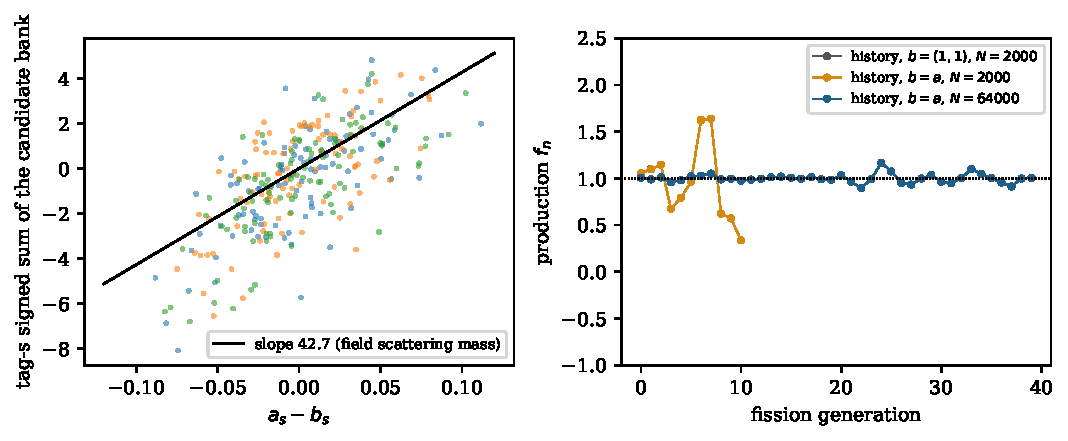
\includegraphics[width=\textwidth]{figures/followup_amplitude_history.pdf}
\caption{Left: signed tag-$s$ sum of the candidate bank against the field's amplitude offset $a_s-b_s$,
for every generation of the three baseline replicas. The slope is the field's scattering production
per unit fission production. Right: the production $f_n$ by fission generation with history-based
flights. With $b=(1,1)$ the run fails at the second generation; with $b=a$ and $N=2000$ it oscillates
and fails; with $b=a$ and $N=64000$ it is stable.}\label{fig:fu:amp}
\end{figure}

\paragraph{History-based flights.} Each flight now continues through its scatterings (37 collisions
per history on average). With $N_\delta=2\times10^4$ histories per generation, the flights cost about
1~s per generation.

\emph{Stability.} With $b=(1,1)$ the iteration fails within two or three generations at $N=2000$ and
at $N=16000$. Damping the normalization ($\lambda=0.1$, $N=4000$) does not save it: all three
replicas fail within eight generations.

The cause is the amplitude term. A fluctuation of $f_n$ puts $42\,(a_s-b_s)$ of scattering mass into
the next residual. A history carries that mass to fission within one generation, at about $0.9$
units of fission production per unit, so the term feeds back on $f$ with a gain of about $40\times0.9$
per unit change of $1/f$, far above one. In the collision iteration the same mass reaches fission over
about 40 generations, and netting and normalization act on it in between.

With $b=a$ the amplitude term is gone. What remains is the residual's own sampling noise, now
delivered to fission in a single generation:
\begin{itemize}
\item at $N=2000$, $f_n$ fluctuates by about $30\%$, and the replicas fail after 11, 22 and 60
  generations;
\item at $N=64000$ ($32\times$ the samples, about one collision generation's worth per collision of a
  history), the run is stable, with:
  \begin{itemize}
  \item $f_n$ varying by $5\%$;
  \item $\Wabs=0.77$;
  \item a lag-1 correlation of $0.50$ ($\tau\approx3$ fission generations);
  \item $k=0.6512$, $+900\pm1100$~pcm, which is not informative;
  \item $47$~s per generation, $95\%$ of it residual sampling.
  \end{itemize}
\end{itemize}

\emph{Figure of merit.} The figure of merit is $2\times10^{-4}$ of the reference, about 9 times
below the collision iteration's $1.8\times10^{-3}$. Per generation, $\sigma_{gen}^2\tau$ is $0.0035$
against $0.0068$. But a generation costs 16 times more, because the residual must be sampled about 30
times more heavily per generation to keep $f_n$ stable.

\emph{What this says about the correlation.} Measured in neutron lifetimes, the collision iteration's
correlation is not long. $\tau=21$ collision generations is about half of a 37-collision lifetime,
while the fission-to-fission iteration has $\tau\approx3$ lifetimes. The apparent long correlation of
Section~\ref{sec:convergence} is long only in units of collision generations, which are cheap. The
real figure-of-merit gap is the variance injected per unit of work, and history-based flights do not
reduce it. They only change when it reaches fission.

\subsection{Toward a speedup: the residual estimator's efficiency}\label{sec:res:speedup}

The follow-up showed that the residual estimator sets the variance. This subsection measures that
estimator's efficiency directly, searches its options, and makes the iteration cheaper. It then
remeasures the whole method. The scans are in \code{examples/rmc/results/speedup}, made by
\code{residual\_efficiency.py}; \code{speedup\_analysis.py} draws the figures.

\paragraph{A measure of efficiency for the eigenvalue.} A generation's residual records enter the bank
and reach fission over the following generations. To first order, their effect on $k$ is their total
fission yield
\begin{equation}
Y=\big\langle 1,\;F\,(I-\mathcal S)^{-1}\hat r\big\rangle=\sum_i w_i\,\eta(\mathbf r_i,E_i),
\end{equation}
with $\eta$ the fission weight that a neutron emitted at $(\mathbf r,E)$ produces in its own
history: an importance for $k$. Two steps build the estimate:
\begin{itemize}
\item $\eta$ is tabulated once, by field region and 60 energy bins, from history flights of
  $2\times10^5$ states;
\item one large sample ($5\times10^4$ to $10^6$ destinations per tag) gives
  $\mathrm{Var}(Y)$ for $N=2000$ records per tag from its per-destination contributions.
\end{itemize}
$\mathrm{Var}(Y)$ times the sampling time measures the eigenvalue noise injected per second. Its
ranking agrees with the full iteration wherever both were measured.

\paragraph{Where the noise is.} In the Stage 8 configuration:
\begin{itemize}
\item the scattering residual carries $97\%$ of $\mathrm{Var}(Y)$; the pooled fission residual
  carries $3\%$;
\item within the scattering residual, fuel destinations above 100~keV account for $44\%$, and fuel
  destinations in the resonance range (4~eV--10~keV) for $36\%$;
\item at $J=8$ directions, about $60\%$ of the variance is direction noise: repeating the same
  destinations with $J=32$ and $J=128$ leaves a floor of $\approx0.011$ (at $N=2000$);
\item at $J=128$ the scattering residual is $4.5\%$ of the field's scattering emission in absolute
  value: $4\%$ in the fuel and $1.2\%$ in the graphite (medians).
\end{itemize}
The largest single contributions come from destinations within $0.01$~cm of the pin surface at
resonance energies, along the one or two directions that look into the graphite. There the
moderator's unshielded flux meets the $^{238}$U scattering resonances.

\begin{figure}[t]\centering
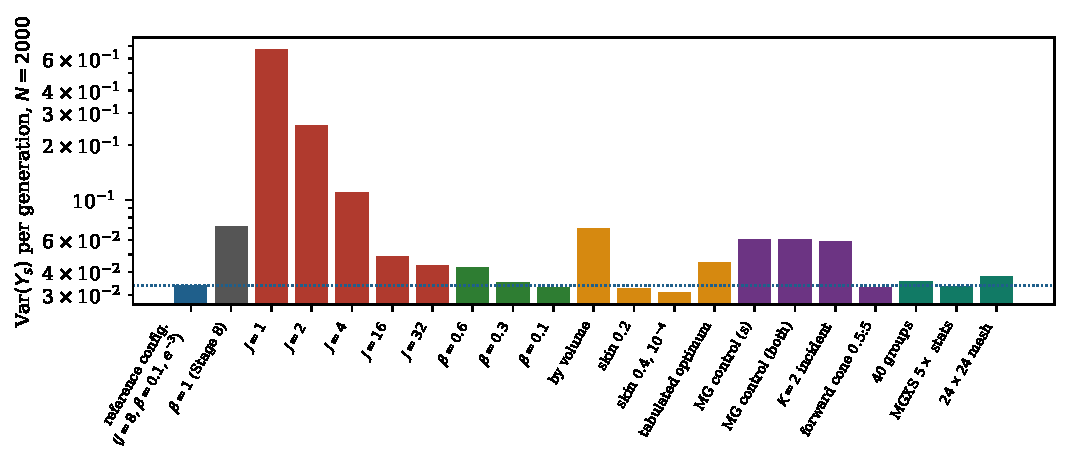
\includegraphics[width=\textwidth]{figures/speedup_scans.pdf}
\caption{Variance of the scattering residual's fission yield per generation ($N=2000$) for the options
tried. The direction, outgoing-energy ($\beta$), destination-by-volume and control scans vary the
Stage 8 settings ($\beta=1$, cutoff $e^{-4}$; variance $0.06$ at $5\times10^4$ samples, $0.07$ at
$10^6$). The skin, tabulated, cone and field scans vary the improved settings ($\beta=0.1$,
cutoff $e^{-3}$; dotted line).}\label{fig:sp:scans}
\end{figure}

\paragraph{What the options do} (Figure~\ref{fig:sp:scans}, Table~\ref{tab:sp:scans}):
\begin{itemize}
\item \textbf{Outgoing-energy proposal.} Drawing 90\% of the outgoing energies from the region's
  emission spectrum ($\beta=0.1$) instead of log-uniformly halves the variance. It also shortens the
  heavy tail: the ten largest of $5\times10^4$ samples carry $12\%$ of the second moment instead
  of $19\%$. This is the one large gain, and it has a second effect, described with the iteration
  below.
\item \textbf{Directions.} The variance falls with $J$ until the floor, and the cost rises with $J$.
  Per unit time, $J=4$ to $8$ is best.
\item \textbf{Destinations.}
  \begin{itemize}
  \item A skin proposal, which draws 20--40\% of the destinations at a log-uniform depth inside the
    pin surface, removes the extreme tail (top-ten share $6\%$) but only $10\%$ of the variance.
  \item A proposal tabulated from a pilot run (region $\times$ 100 energy bins,
    $\propto\sqrt{n_b\,m_{2,b}}$) is worse. Its bins are far wider than the resonances, so it
    misplaces the samples within them.
  \end{itemize}
\item \textbf{Controls.} The MG control on the same paths, more incident energies on the sampler
  route, and a forward cone of directions for forward-peaked fast kernels leave the variance
  unchanged or raise it. The MG control's production tracks the CE production closely overall
  (correlation $0.99$), but not where the variance is: at the CE fine structure in energy.
\item \textbf{The field.} 40 groups instead of 8, five times the MGXS statistics, or a $24\times24$
  source-region mesh leave the variance unchanged. Within these options, neither the group
  structure, the MGXS noise, nor the spatial resolution sets the residual's noise. Material-level
  lifts and isotropic flat emission are what the field cannot represent near the pin surface.
\end{itemize}

\begin{table}[t]\centering\small
\caption{Variance of the residual's fission yield per generation ($N=2000$ per tag) for each option:
scattering ($s$) and fission ($f$), and the share of the scattering second moment carried by the
ten largest samples.}\label{tab:sp:scans}
\begin{tabular}{@{}llrrr@{}}
\toprule
group & option & Var$(Y_s)$ & Var$(Y_f)$ & top ten\\
\midrule
\csname @@input\endcsname figures/speedup_scans.tex
\bottomrule
\end{tabular}
\end{table}

\paragraph{Engineering.} A residual sample's time is spent tracing backward paths: geometry, mesh
crossings, cross sections and attenuation. Four changes make the scattering residual $3.5$ times
faster (1.07~s to 0.31~s per 2000 samples), with identical results:
\begin{itemize}
\item a per-path cache of $\Sigma_t$ for each energy and material state, since a path alternates
  among few materials;
\item the field's energy bins found once per energy instead of once per segment;
\item dense region tables per meshed cell instance, instead of hash lookups;
\item an incremental regular-mesh traversal (Amanatides--Woo) in place of OpenMC's general
  \code{bins\_crossed}, and one transcendental function per segment and energy instead of two.
\end{itemize}
The per-generation correction tally is not needed for $k$. Its field part is the same every
generation up to the amplitudes, so it can be computed once. The $k$ runs below omit it.

\begin{table}[t]\centering\small
\caption{The iteration after the changes of this subsection, against the reference. The columns are:
the number of replicas; $\Delta k$ with its standard error, from 10-generation batch means pooled over
the replicas; $\overline{\Wabs}$; the per-generation spread of $k_n$; the active time per replica; and
the $k$ figure of merit relative to OpenMC (replica spread of the reference). Unless stated
otherwise, every run uses $N=2000$ per tag, $N_B=4\times10^4$, 40 inactive and 60 active
generations, and the combined cancellation.}\label{tab:sp:runs}
\setlength{\tabcolsep}{3.5pt}
\resizebox{\textwidth}{!}{%
\begin{tabular}{@{}lrrrrrr@{}}
\toprule
run & $n$ & $\Delta k$ (pcm) & $\overline{\Wabs}$ & $\sigma_{gen}$ & $T$ & FOM$_k$\\
\midrule
\csname @@input\endcsname figures/speedup_runs.tex
\bottomrule
\end{tabular}}
\end{table}

\paragraph{The iteration, remeasured} (Table~\ref{tab:sp:runs}). With $b=a$, $\beta=0.1$, a cutoff of
$e^{-3}$, $N_\delta=5\times10^4$ and the faster tracer:
\begin{itemize}
\item \textbf{Bias.} The eigenvalue bias at $N=2000$ falls from $+900$ to between $+120$ and
  $+600$~pcm, depending on the seeds. Nine independent replicas of these settings (one set of three with smaller banks) give
  $+350\pm125$~pcm.
\item \textbf{Correlation.} The integrated autocorrelation time falls from $\approx21$ generations to
  $\approx3$.
\item \textbf{Figure of merit.} It rises from $0.005$ to $0.08$--$0.12$ of OpenMC's (batch-means
  errors on both sides of the change), about $20$ times.
\end{itemize}

Ablations with paired seeds (3000--3002) tie the change in bias to the energy proposal: the baseline
gives $+900$~pcm, $b=a$ with the cutoff $e^{-3}$ gives $+1130$, and $b=a$ with $\beta=0.1$ gives $-75$. The log-uniform proposal's
heavy tail, a few samples carrying a large share of the second moment, did two things:
\begin{itemize}
\item it drove the long excursions of $k_n$ that made the error estimates so different;
\item through the iteration's nonlinear normalization, it produced most of the bias.
\end{itemize}

At $N=8000$ the per-generation spread halves, and the figure of merit is $0.08$--$0.17$, depending on
the replicas.

\paragraph{The remaining bias.} At $N=8000$ the error of $k$ is small enough to expose a systematic
offset. Six replicas give $+950\pm70$ and $+1070\pm100$~pcm (field placement).
Figure~\ref{fig:sp:bias} shows how it builds up: $k_n$ starts near the reference while the bank is
empty and rises over 20--30 generations, the time the scattering correction takes to reach fission.
Several observations constrain its cause:
\begin{itemize}
\item \textbf{Placement.} Re-sampling netted particles from the bin's own particles of the net's sign
  ('empirical' placement) lowers it to $+660\pm100$~pcm. Finer netting bins (12$\times$12 zones, 4
  sub-bins per group) lower it to $+690$ (one replica).
\item \textbf{Frequency.} Netting every second or fourth generation does not lower it in proportion
  ($+985$ and $+650$, one replica each).
\item \textbf{No netting.} Without netting the bank's absolute weight grows by the residual's injection
  every generation (about 7 units), and the run fails after 65 generations.
\item \textbf{The residual.} The scattering residual's mean fission yield from $10^6$ samples is
  $+0.006\pm0.009$ (density route), $-0.002\pm0.044$ (density-free) and $+0.016\pm0.012$
  ($\beta=1$). The routes agree, so no bias of the residual is visible at that precision.
\end{itemize}
So netting's projection explains part of the bias, but not all of it. Which other part of the
iteration contributes is the next question.

\begin{figure}[t]\centering
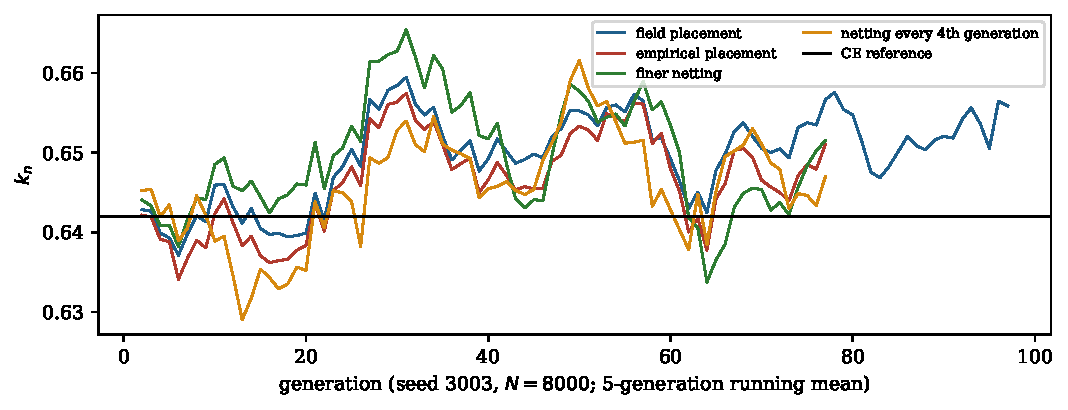
\includegraphics[width=\textwidth]{figures/speedup_bias_buildup.pdf}
\caption{$k_n$ by generation at $N=8000$ for four cancellation settings with the same seed (5-generation
running means). The runs share their residual samples, so their fluctuations coincide. $k_n$ starts
near the reference while the bank is empty, and rises over the 20--30 generations the scattering
correction needs to reach fission. Empirical placement and finer netting lower the plateau, but do not
remove it.}\label{fig:sp:bias}
\end{figure}

\paragraph{How far from a speedup.} The best configurations reach $0.1$--$0.17$ of analog Monte Carlo's
figure of merit for $k$, a factor of 6--10 short of break-even. The remaining levers:
\begin{itemize}
\item \textbf{Fixed costs.} Python-side cancellation (about 20\% of a generation) and bank handling
  could be moved to C++, a factor of about 1.3.
\item \textbf{Larger $N$.} Amortizing the fixed costs further gives at most 1.5.
\item \textbf{Fewer directions per unit of noise.} A per-stratum allocation of directions, more where
  direction noise dominates (fuel above 10~keV), gives an estimated 1.2--1.5.
\end{itemize}
These multiply to about 3. Closing the rest needs a residual that is smaller where it matters: lifts
resolved in space near the pin surface, or an anisotropic field emission. The measurements bound how
small it must be. A scattering residual that is a fraction $\varepsilon$ of the scattering emission
has an absolute fission yield of about $\varepsilon\,\bar n_c$ per unit of fission production, with
$\bar n_c\approx37$ the number of collisions in a neutron's life. With $\varepsilon\approx4.5\%$
here, that is about 1.7: larger than the production itself. The method beats analog Monte Carlo only
when $\varepsilon\,\bar n_c\ll1$. In graphite that means a field accurate to well below 1\% locally;
in light water, with $\bar n_c\approx20$, about twice that.

\subsection{Resonance-resolved lifts and several energies per trace}\label{sec:res:lifts}

The speedup study ended with two open items: a bias of $+650$ to $+1000$~pcm, and a scattering
residual too noisy by a factor of 6--10. This subsection finds the cause of the first, makes the
scattering residual about five times more efficient, and finds that a different term now limits
the method. The runs are in \code{examples/rmc/results/speedup2}.

\paragraph{What the direction noise is.} Anisotropic emission was to be the next field improvement.
Before implementing it in random ray, its potential was measured. The scattering residual was
evaluated at fixed destinations and energies for 12 outgoing directions (128 incident directions
each), and split into its angle average and the rest:
\begin{itemize}
\item the angular part carries $15\%$ of the residual's second moment overall;
\item in the fuel it carries $13\%$, and in the fast fuel about $1\%$.
\end{itemize}
An anisotropic field could remove at most that share, so it was not implemented.

The per-direction data show what the noise is instead. At a fixed destination and outgoing state,
the CE production of single incident directions scatters by $13$--$100\%$ about its mean. The MG
production on the same paths varies by about $5\%$ and is uncorrelated with it. Each direction has
its own image energy $E'=E/\gamma_A(\mu_0)$ for each nuclide, and the path's flux $\psi(E')$ has
resonance structure: a ray that crosses the pin at an energy on a $^{238}$U resonance arrives
attenuated, and a neighbouring energy does not. The direction noise is therefore noise in
\emph{energy}, sampled once per direction. No smooth control can follow it. Three were tried:
\begin{itemize}
\item a control with the region's isotropic flux at the same image energies: correlation $0.95$ in
  the fast fuel, where the structure is the kernel's and not the flux's, but only $-25\%$ in the
  total variance;
\item a control with the local uncollided flux $Q/\Sigma_t$: no gain;
\item incident directions drawn from a learned distribution of the scattering cosine: $-15\%$.
\end{itemize}

\paragraph{Several outgoing states per destination.} If the noise is in energy, more energies per
trace average it. Each destination now carries $K_{out}$ outgoing states (energy and direction), each
a density record of its own, and all of them share the destination's $J$ backward traces: the image
energies of every state ride on each path. Three details matter:
\begin{itemize}
\item \textbf{Stratified energies.} The $K_{out}$ energies are stratified over the proposal
  (systematic sampling with one random offset), so every destination covers the energy range. This
  matters in the fast fuel: there the sampler-route particles (inelastic scattering) of a
  destination are offset by the low term at fast outgoing energies, and only on average.
\item \textbf{Image roulette.} In the fuel each state has one image per nuclide, and trace nuclides
  contribute little. Nuclide $n$'s image is kept with probability
  $p_n=\min(1,\max(0.25,4\times\text{its share of }\Sigma_s))$ and weighted by $1/p_n$. A floor of
  $0.05$ is too low: a rare image on a resonance then carries a weight of 20.
\item \textbf{Tabulated incident energies} for the sampler route, proportional to its production
  times the lifted flux. A log-uniform draw over twelve decades mostly misses the inelastic
  thresholds.
\end{itemize}
The estimate stays unbiased for any $K_{out}$: every record carries $K_{out}$ times its draw density.

\begin{table}[t]\centering\small
\caption{The scattering residual with $K_{out}$ outgoing states per destination ($J=8$, $\beta=0.1$,
cutoff $e^{-3}$, $N=2000$ destinations): variance of the fission yield per generation and time per
generation. The last column is their product relative to $K_{out}=1$ with the first lifts.}
\label{tab:lifts:ko}
\begin{tabular}{@{}llrrr@{}}
\toprule
lifts & $K_{out}$ & Var$(Y_s)$ & time (s) & Var $\times$ time\\
\midrule
200 fine bins per group & 1 & 0.0338 & 0.32 & 1\\
 & 4 (independent energies) & 0.0103 & 0.68 & 0.65\\
 & 8 (stratified, roulette, tabulated incident) & 0.0059 & 0.93 & 0.51\\
 & 16 & 0.0028 & 1.43 & 0.37\\
resonance-resolved (4000 bins, 4~eV--5.5~keV) & 1 & 0.0290 & 0.31 & 0.83\\
 & 8 & 0.0043 & 0.96 & 0.38\\
 & 16 & 0.0023 & 1.49 & 0.32\\
\bottomrule
\end{tabular}
\end{table}

The variance falls nearly as $1/K_{out}$ (Table~\ref{tab:lifts:ko}), almost as if each state were an
independent destination, while a state costs about a sixth of a destination. With $K_{out}=16$ and the
lifts below, the scattering residual's variance at equal time is about a third of what it was. In the
iteration, the bank's absolute weight falls below one for the first time ($\Wabs\approx0.85$).

\paragraph{Resonance-resolved lifts remove the bias.} The lifts had 200 fine bins per group. In the
group from 4~eV to 5.5~keV that is a lethargy width of $0.036$ per bin, ten times wider than the
$^{238}$U resonances. The scattering emission of the fuel keeps resonance structure, because a
collision with $^{238}$U changes the lethargy by at most $0.017$. So the low term $U(E)$ averaged
over structure that the CE production $C(E)$ resolves, and the residual in the fuel carried large
positive and negative parts within every lift bin.

New lifts were tallied with 4000 bins in that group (lethargy width $0.0018$) and 800 in the next.
The field's group emission is unchanged; only the within-group shapes are finer. Two results:
\begin{itemize}
\item \textbf{Variance.} The scattering residual's variance falls by $15$--$30\%$
  (Table~\ref{tab:lifts:ko}).
\item \textbf{Bias.} With the same seeds and settings ($N=8000$, $K_{out}=1$, empirical placement),
  the bias goes from $+664\pm102$~pcm to $-31\pm80$~pcm (the error from batch means; the three
  replicas agree within $30$~pcm). With $K_{out}=16$, nine replicas give $-86\pm58$~pcm.
\end{itemize}
This settles the cause of the bias. It was netting: not through the netting bins of the resonance
range, which the follow-up tested, but through what was in them. The unresolved low term made the
correction carry large cancelling parts on the scale of single resonances, and every netting
smeared them within its bins. With lifts that resolve the resonances, the correction no longer has
that structure, and netting's projection error falls below the present precision of about 80~pcm.

\paragraph{What limits the method now.} With the scattering residual quieter, the figure of merit
should have risen. It did not: the best configuration ($K_{out}=16$, resonance-resolved lifts,
$N=2000$, $N_f=6000$) gives $\sigma(\bar k)=0.0013$--$0.0017$ over 60 generations in about 145~s. That
is a figure of merit of $0.09$--$0.16$ of OpenMC's, the same as before within its uncertainty.

The reason is a noise source that had been hidden. The per-generation spread of $k_n$ is now white
(no autocorrelation) and proportional to $1/\sqrt{N_f}$, the number of \emph{fission} residual
samples:
\begin{center}\small
\begin{tabular}{@{}lrr@{}}
\toprule
run & $N_f$ & $\sigma_{gen}$\\
\midrule
$N=2000$, $K_{out}=8$ & 2000 & 0.0168\\
$N=4000$, $K_{out}=8$ & 4000 & 0.0126\\
$N=2000$, $K_{out}=16$ & 6000 & 0.0095\\
$N=8000$, $K_{out}=1$ & 8000 & 0.0088\\
\bottomrule
\end{tabular}
\end{center}
This is the noise of one number: the CE fission production of the field's own first-flight flux,
\begin{equation}
X=\big\langle\nu\Sigma_f,\;\phi^{CE}[a\,\Qmg]\big\rangle,
\end{equation}
which enters every $k_n$ through the fission residual's mass. $X$ is a constant of the frozen field.
Estimating it directly and averaging the estimates over the generations
(\code{-{}-field-production}) removes the white noise: $\sigma_{gen}$ falls from $0.0095$ to
$0.003$. But the error of the running mean is then shared by every generation, and the spread of
replica means stays at $0.002$.

The eigenvalue cannot be known better than $X$: $\sigma_k/k\ge\sigma_X/X$. And $X$ is expensive to
estimate, because no variance reduction is in place for it:
\begin{itemize}
\item the MG control on the same paths lowers its variance only from $(1.7\%)^2$ to $(1.2\%)^2$ per
  $2\times10^4$ points;
\item for the fission residual, more incident energies or directions per sample lower the variance
  only in proportion to their cost (Var $\times$ time is constant from 8 to 256 path-energies per
  sample).
\end{itemize}
Reaching the reference's $0.077\%$ in $X$ with the present estimator takes about as long as the
reference itself. This term, not the scattering residual, now sets the figure of merit.

\paragraph{Where a speedup has to come from.} The method's premise holds for the shape of the
correction: it is carried by signed particles whose absolute weight is now below the fission
production. It does not yet hold for the one scalar $X$, which is estimated at analog-like cost. The
candidates:
\begin{itemize}
\item \textbf{A correlated control for $X$.} Evaluate the CE and the lifted-MG fission production
  at the same incident energies on the same path, $\nu\Sigma_f(E')\,[\psi^{CE}(E')-\psi^{MG}_{g}h_\phi(E')]$,
  so that only the flux difference is sampled. The flux-difference control of the sampler route did
  this for the high term of the fission residual (4.7 times, Section~\ref{sec:res:controlled}); it
  has to be combined with destination pooling.
\item \textbf{Importance in the thermal range.} Most of $X$ is thermal fission in the pin's outer
  layer. Destinations by the field's fission emission and incident energies by
  $\nu\Sigma_f\phi$ are not yet used for tag $f$.
\item \textbf{A field that carries $X$.} If the MG cross sections were condensed with the CE flux of
  the field's own emission, the MG and CE fission productions of the field would agree by
  construction, and $X-X^{MG}$ would be a second-order quantity.
\end{itemize}

\subsection{The field's fission production, the eigenvalue update, and exact cancellation}\label{sec:res:X}

Section~\ref{sec:res:lifts} left one scalar as the limit: $X$, the CE fission production of the
field's first-flight flux. This subsection removes that limit, finds the next one in the eigenvalue
update itself, and answers two questions about cancellation. The runs are in
\code{examples/rmc/results/speedup3}.

\paragraph{An importance-sampled estimator of $X$.} The estimators so far drew backward points
uniformly in space and incident energies from the lifted flux. The score
$\nu\Sigma_f(E')\,\psi(E')/p$ then varies by orders of magnitude, with the $1/v$ cross section and
the fission resonances. The new estimator (\code{field\_fission\_production}) draws from the field's
own lifted fission rate on the lifts' fine grid:
\begin{equation}
p(\mathbf r,E')\;\propto\;\phi_{R,g(E')}\,h_\phi(E')\;\nu\Sigma_f(E'_i),\qquad \mathbf r\in R,\ E'\in\text{fine bin }i,
\end{equation}
with an isotropic direction. The score is then the total of those weights times two ratios near
one: the CE $\nu\Sigma_f$ at $E'$ to its value at the bin's midpoint, and the path's CE angular
flux to the region's lifted scalar flux per unit solid angle. It is unbiased for any lifts, because
the density is evaluated exactly.

\begin{center}\small
\begin{tabular}{@{}lrr@{}}
\toprule
estimator of $X$ & relative error $\times\sqrt{\text{seconds}}$ & variance $\times$ time\\
\midrule
uniform points, energies from the lifted flux & 0.87\% & 1\\
the same with the MG control on the path & 0.61\% & 0.5\\
lifted fission rate, 4 energies per point & 0.071\% & 1/150\\
lifted fission rate, 16 energies per point & 0.057\% & 1/230\\
\bottomrule
\end{tabular}
\end{center}
With the resonance-resolved lifts, the reference's $0.077\%$ is reached in about one second. With
the 200-bin lifts the gain is only about 9 in variance: the fission resonances must be resolved by
the proposal. In the iteration, $X$ is estimated with 5000 points per generation and averaged over
the generations (0.13~s per generation).

\paragraph{The white noise is gone; a long memory remains.} With this estimate, the per-generation
spread of $k_n$ falls from $0.0095$ to $0.0024$. But the spread of the replica means is also
$0.0024$ (six replicas, 60 active generations each): within a replica, the deviation of $k_n$
persists for the whole active phase. The lag-1 autocorrelation is $0.6$--$0.7$.

The cause is the eigenvalue update, not an estimator. In the emission-source form
$k_{n+1}=k_nf_n$, and the fission emission is rebuilt with $1/k_{n+1}$. An error in $k_n$
therefore changes the fission-born source at once, but the production $f$ responds only when
those neutrons have slowed down and caused fission, about one neutron lifetime (37 collision
generations) later. The loop that corrects $k$ has a delay of a lifetime, so $k_n$ carries every
past fluctuation for tens of generations. A 60-generation active phase then holds only two or
three independent values of $k$. With $\sigma(\bar k)=0.0024$ in 118~s, the figure of merit
is about $0.06$--$0.4$ of OpenMC's, depending on the error estimate, and no better than before on
the replica estimate.

\paragraph{History-based flights, revisited.} A fission-to-fission generation closes that loop within
one generation, and its bank is small. With the present estimators the history-based iteration is
stable at $N=2000$ (it needed $N=64000$ in Section~\ref{sec:res:followup}), with
$\Wabs\approx1.1$. But $k_n$ now oscillates with a period of about six generations and an amplitude
of $\pm15\%$ (autocorrelation $+0.5$, $-0.4$, $-0.8$ at lags 1--3), and the replica means scatter by
$0.005$. Two normalization variants were tried:
\begin{itemize}
\item fixed amplitudes $b=(1,1)$: fails within four generations, as before;
\item damped normalization ($\lambda=0.3$): the per-generation spread falls from $0.10$ to $0.033$,
  but the oscillation and the replica spread ($0.006$) remain.
\end{itemize}
The oscillation comes from the same update. With following amplitudes, $a_{s}$ and $a_f$ are
integrators ($a_{s,n+1}=a_{s,n}/f_n$, $a_{f,n+1}=a_{f,n}/f_n^2$), and $k_n$ is a third. In history
mode their restoring forces act with a delay of one or two generations and a gain near one: an
underdamped loop. So the fission-to-fission bank is cleaner, as expected, but the per-tag
normalization of Section~\ref{sec:iteration} is the wrong controller for it.

\paragraph{What to change next.} The estimators are no longer the limit: the scattering residual,
$X$ and the bank are each well below the present error. The limit is the controller that turns
them into $k$. Section~\ref{sec:res:grouped} implements an eigenvalue estimate without that memory,
and the exact cancellation at fission births that this section had left open.

\subsection{Grouped cancellation at fission births, and a balance eigenvalue}\label{sec:res:grouped}

This subsection implements two things and measures each: the exact grouped cancellation at fission
births of the companion proposal, and an eigenvalue update without memory. The runs are in
\code{examples/rmc/results/speedup4}.

\paragraph{Grouped cancellation: the estimator.} A bank entry is either a directional particle or an
\emph{emission record} $w_j\,\delta_{\mathbf x_j}P_j$: a site with an emission law that has not been
sampled yet as far as the estimator is concerned. Two laws are implemented:
\begin{itemize}
\item a fission birth: isotropic, at its sampled energy $e_j$;
\item an elastic scattering off a stationary target (incident energy above $400\,kT$): the record
  keeps the incident energy $\varepsilon_j$, the incident direction $\Omega_j$ and the nuclide. In a
  direction $\mathbf d$, with $\mu=\Omega_j\!\cdot\!\mathbf d$, the outgoing energy is
  $e_j=\varepsilon_j\,\gamma_A(\mu)$ and the density per solid angle is
  $p_{\text{lab}}(\mu\,|\,\varepsilon_j)/2\pi$.
\end{itemize}
Every other entry is directional: fresh residual particles, inelastic and thermal scatterings.
Groups are fixed from the incoming bank before the flights (records sorted by zone, law and energy
decade, in runs of $G$). A flight that causes fission at
$y=(\mathbf x,\ \text{nuclide }\ell,\ E_f)$ after a path shorter than $d_{\max}$ gets the weight
\begin{align}
W_G(y)&=\frac{\sum_{j\in G}J_j(y)}{\sum_{j\in G}m_j\,q_j(y)},\qquad
J_j=\frac{w_j\,\nu_\ell(e_j)}{k}\,q_j ,\\
q_j(y)&=\sum_{\text{paths}}a_j(\mathbf d)\,\frac{e^{-\tau(e_j)}}{r^2}\,\sigma_{f,\ell}(e_j)\,\chi_\ell(E_f\,|\,e_j),
\end{align}
with $m_j=N_\delta|w_j|/\Wabs$ the expected number of flights of member $j$, and the sum over the
reflected paths shorter than $d_{\max}$. A group of one gives back the ordinary weight. The code is
\code{rmc::grouped\_fission\_weight} and \code{GroupedFissionCancellation}
(\code{examples/rmc/cancellation.py}).

\paragraph{It is exact.} Gate G8.10 flies 2000 signed parents once, turns the children into
records, flies them again, and compares the fission grandchildren's weight in four bins of emitted
energy with ordinary and with grouped weights, over 120 repetitions of both flights. The paired
differences are $0.1$, $-1.4$, $0.7$ and $0.6$ standard errors, and a standard error is $0.7$--$1.1\%$
of the eligible weight per bin. The eligible absolute weight falls from $59.9$ to $23.5$ with $G=8$.

\paragraph{It is not sufficient.} Table~\ref{tab:res:grouped} gives the tuned configuration of
Section~\ref{sec:res:X}, without and with netting.

\begin{table}[t]\centering\small
\caption{Grouped cancellation at fission births ($G=32$, $d_{\max}=3$~cm). Without netting: one
replica, generation 7. With netting: three replicas, 60 active generations, same seeds in both
rows.}\label{tab:res:grouped}
\begin{tabular}{@{}lrrrrr@{}}
\toprule
 & $\Wabs$ & fission births & eligible & eligible $\sum|w|$ & all fission $\sum|w|$\\
\midrule
no netting, regional kernel & $52.7$ & & & & \\
no netting, grouped & $50.5$ & 248 & 105 & $0.383\to0.095$ & $0.92\to0.63$\\
netting, regional kernel & $0.94$ & 438 & 41 & & \\
netting, grouped & $0.95$ & 438 & 32 & $0.0026\to0.0021$ & $0.0349\to0.0345$\\
\bottomrule
\end{tabular}
\end{table}

\begin{itemize}
\item \textbf{Without netting the bank grows as before}: by $6.4$ in absolute weight per generation,
  with or without grouping. Grouping removes three quarters of the eligible fission weight, but
  fission births carry $2\%$ of the bank's weight. The scattering children carry the rest, and the
  method does not act on them: two members reach a site with different incident states, and their
  scattering laws there lie on different kinematic surfaces.
\item \textbf{Only a minority of fission births are eligible}: $42\%$ without netting and $7\%$
  with it. In this lattice most fission is thermal, and its parent is a thermal scattering in
  graphite. That law is tabulated with discrete outgoing angles and has no density to evaluate.
  With netting, most of the remaining weight is fresh residual particles, which are directional.
\item \textbf{With netting it changes nothing measurable}: $k=0.63925$ against $0.63920$ on the
  same seeds, and a replica spread of $0.0025$ against $0.0026$.
\end{itemize}
So the answer to ``is it sufficient for weight cancellation'' is no, for a structural reason: the
weight that must cancel is scattering weight. The grouped estimator is kept as an exact, tested
component (it generalizes the regional kernel of Section~\ref{sec:cancellation}, which is the
special case of isotropic members); it would matter in a fast system, where fission births follow
elastic or fission-born parents.

\paragraph{A balance eigenvalue.} The update $k_{n+1}=k_nf_n$ measures the eigenvalue through the
growth of the fission production from one generation to the next. In a collision-by-collision
iteration that growth is $1+(k/k_n-1)/\Lambda$ with $\Lambda\approx37$ collisions per lifetime, so a
generation corrects $1/\Lambda$ of the error in $k_n$ and the noise of $\Lambda$ generations
accumulates in it. The balance of one generation's flux has no such factor:
\begin{equation}
k^{\text{bal}}_n=\frac{P_n}{L_n},\qquad
P_n=\langle\nu\Sigma_f\,\phi_n\rangle,\qquad
L_n=\langle\Sigma_a\,\phi_n\rangle-\langle\text{gain of multiplying scatterings}\rangle .
\end{equation}
For the eigenfunction of the iteration run with a wrong $k_n$ (growth $\lambda$ per generation, tag
masses $M_s$, $M_f$), $L=M_f+(1-\lambda)M_s$ and
$k^{\text{bal}}\approx k_n\,(1+(\lambda-1)(1+M_s/M_f))=k_n(1+\Lambda(\lambda-1))$: the full correction
in one generation, from tallies whose noise is not multiplied by $\Lambda$. The pieces are:
\begin{itemize}
\item the field's part of $L$, $a_sL_s+a_fL_f$: two constants of the frozen field like $X$,
  estimated by the same importance-sampled backward estimator with the net loss cross section
  (\code{field\_production(score='loss')}; $\Sigma_t$ minus the production of every non-fission
  channel) and averaged over the generations;
\item the bank's part of $L$ and of $P$: collision estimators over the flights
  ($w\,\Sigma_a/\Sigma_t$ and $w\,\nu\Sigma_f/\Sigma_t$ at every collision, less the analog gain of
  multiplying scatterings), in place of counting about 440 analog fission births;
\item the update: both tags are normalized by $P_n$ alone, and
  $k_{n+1}=\sum P/\sum L$ over the last 20 generations. The run's estimate is $\sum P/\sum L$ over
  the active generations.
\end{itemize}
On the four-region toy the balance update converges to the CE eigenvalue with less than half the
error of the production update in each of the first five generations (\code{test\_driver\_toy.py}).

\paragraph{Result.} Table~\ref{tab:res:balance} compares the updates in the tuned configuration
($K_{out}=16$, resonance-resolved lifts, $N_\delta=5\times10^4$, 40 inactive and 60 active
generations). The error of a replica is the spread of the replica estimates, the measure on which
Section~\ref{sec:res:X} found $0.05$.

\begin{table}[t]\centering\small
\caption{The eigenvalue with the production update and with the balance update. $\Delta k$ against
the analog reference ($\sigma=0.00049$ in 151~s). FOM is $1/(\text{spread}^2\,T)$ relative to the
reference, with the 68\% interval that the number of replicas allows.}\label{tab:res:balance}
\setlength{\tabcolsep}{4pt}\footnotesize
\begin{tabular}{@{}lrrrrrrl@{}}
\toprule
update, configuration & repl. & $\Delta k$ (pcm) & spread & per gen. & lag-1 & $T$ (s) & FOM\\
\midrule
production, $N=2000$ & 9 & $-86\pm58$ & 0.0024 & 0.0024 & 0.6--0.7 & 118 & 0.05\\
balance, $N=2000$ & 10 & $-42\pm32$ & 0.00102 & 0.0027 & 0.34 & 133 & 0.26 (0.14--0.38)\\
balance, $N=8000$ & 6 & $+17\pm38$ & 0.00092 & 0.0017 & 0.56 & 410 & 0.11 (0.04--0.17)\\
balance, $N=1000$, $10^4$ loss pts. & 18 & $-113\pm25$ & 0.00107 & 0.0040 & 0.27 & 100 & 0.32 (0.22--0.43)\\
the same, damping $\lambda=0.2$ & 12 & $-91\pm28$ & 0.00098 & 0.0042 & 0.28 & 93 & 0.41 (0.24--0.58)\\
balance, history flights & 2 of 3 & $+39\pm41$ & & 0.0051 & $-0.08$ & 395 & \\
\bottomrule
\end{tabular}
\end{table}

\begin{itemize}
\item \textbf{The memory of the update is gone.} The replica spread falls from $0.0024$ to $0.0010$
  at the same cost, and the lag-1 autocorrelation from $0.6$--$0.7$ to $0.3$. The figure of merit
  on the replica measure rises from $0.05$ to $0.26$ of OpenMC's, a factor of five.
\item \textbf{It is still below one.} The spread is three times what independent generations would
  give ($0.0027/\sqrt{60}=0.00035$). What remains is correlated over about eight generations and is
  not the residual's sample size: at $N=8000$ the per-generation spread falls to $0.0017$ but the
  replica spread does not move, and at $N=1000$ it does not rise.
\item \textbf{The field's net loss is now the least precise constant.} Its estimator reaches
  $0.27\%\cdot\sqrt{\text s}$, against $0.066\%\cdot\sqrt{\text s}$ for $X$: $69\%$ of the loss is
  resonance absorption in the fuel, where the path's angular flux differs from the lifted flux by a
  factor of order one (relative spread $1.0$ per point). With 5000 points per generation its
  running mean contributes about $0.0006$ to a replica's error, a third of the variance; with
  $10^4$ points, about $0.0004$.
\item \textbf{A bias appears at small $N$.} $-113\pm25$~pcm at $N=1000$, $-42\pm32$ at $N=2000$,
  $+17\pm38$ at $N=8000$: consistent with a term proportional to $1/N$. It does not come from
  dividing by the noisy production: damping the normalization to $P_n^{0.2}$ leaves it at
  $-91\pm28$ on the same seeds. Its origin is not identified; the candidates are the netting of a
  noisier candidate bank and the following amplitudes $b=a$, which multiply the residual's noise.
\item \textbf{History flights.} With the balance estimate, the per-generation spread of the
  eigenvalue is $0.005$ where $k_nf_n$ oscillated by $\pm15\%$, so the controller was indeed the
  cause of the oscillation. But the fission-to-fission bank is not netted: in one of three replicas
  it grew from $\Wabs=9$ to $106$ in eight generations and the production turned negative. At
  $5.5$~s per generation it is also three times as expensive.
\end{itemize}

\paragraph{Where this leaves the method.} The best unbiased configuration is the balance update at
$N=2000$: $\Delta k=-42\pm32$~pcm and a figure of merit of $0.26$ ($0.14$--$0.38$) of analog Monte
Carlo, from $0.05$. No speedup is demonstrated. The remaining factor of four has two identified
parts:
\begin{itemize}
\item the net loss of the field's flux, which needs an estimator for resonance absorption as good as
  the one for fission (a proposal that follows the self-shielded angular flux, or lifts by zone);
\item the correlated part of the bank's production and loss, which neither $N$ nor the
  normalization changes. The bank's flights ($N_\delta$), its compression ($N_B$) and the netting
  are the untested suspects.
\end{itemize}

\subsection{The field's constants, and where the figure of merit stands}\label{sec:res:constants}

Section~\ref{sec:res:grouped} named two limits, and this subsection measures both. The run data are
in \code{examples/rmc/results/speedup5}.

\paragraph{How much of the error is the constants.} A balance run estimates the field's production
$X$ and net loss $L$ as running means. The final running mean of each replica can be recovered
from its rows, and the replica estimates recomputed with the mean over all replicas in its place:
\begin{center}\small
\begin{tabular}{@{}lrrrr@{}}
\toprule
 & replicas & spread as run & with pooled $X$, $L$ & spread of $\hat L_s$ (relative)\\
\midrule
$N=1000$ & 18 & 0.00107 & 0.00080 & 0.063\%\\
$N=2000$ & 10 & 0.00102 & 0.00062 & 0.073\%\\
$N=8000$ & 6 & 0.00092 & 0.00020 & 0.091\%\\
\bottomrule
\end{tabular}
\end{center}
The net loss of the field is most of a replica's error at $N=8000$ and a large part at
$N=2000$. Its relative error is $-\delta L/L$ in $k$, because the field carries $99\%$ of the
absorption.

\paragraph{The loss estimator cannot be improved by a better energy proposal.} The estimator's error
is $0.28\%\cdot\sqrt{\text s}$, and its variance per point is $0.06+0.85/n_E$ with $n_E$ energies
per path: the energies are already at their optimum. The loss is $69\%$ in the group from 4~eV to
5.5~keV and $24\%$ in the next one. At a resonance peak the path's flux over the lifted flux is
$0.3$ for a path from inside the fuel and $12$ for a path that enters through the rim. Two proposals
that follow this structure were implemented (\code{field\_production(hyperfine=...)}):
\begin{itemize}
\item energies from bins of lethargy width $10^{-4}$ (or $3\times10^{-5}$) weighted with the
  narrow-resonance flux $\Sigma/(\Sigma_t+\sigma_e)$;
\item the same bins sorted into 16 classes of $\Sigma_t$, with the class chosen by the flux that a
  path with $d$ cm of fuel behind it would see,
  $W_c\,[(1-e^{-S_cd})/S_c+e^{-S_cd}/\sigma_e]$.
\end{itemize}
Neither changes the error ($0.28$--$0.30\%\cdot\sqrt{\text s}$), and the roulette cutoff does not
either ($e^{-3}$, $e^{-5}$, $e^{-8}$). The proposal's tables are now built once per field instead of
at every call. So the constants are computed before the run (\code{field\_constants.py},
\code{stage8.py --field-constants}): $L_s=1.5293$ and $X_s=0.9336$ to $0.01\%$, in about 1100~s for
$L$ and 150~s for $X$; two independent sets with hashed seeds agree ($1.5292\pm0.0003$,
$1.5297\pm0.0003$).

\paragraph{With the constants fixed.} Table~\ref{tab:res:constants} gives the balance iteration at
$N=8000$ with $J=4$, 8 and 16 directions per destination. With six replicas the spread is uncertain, so the
error of a replica is also estimated from batch means of 20 generations pooled over the replicas.

\begin{table}[t]\centering\small
\caption{The balance iteration with precomputed constants, $N=8000$, $N_f=2000$, six replicas.
FOM relative to the analog reference; the time of the constants is not included.}\label{tab:res:constants}
\setlength{\tabcolsep}{4pt}\footnotesize
\begin{tabular}{@{}lrrrrrrr@{}}
\toprule
 & $\Delta k$ (pcm) & spread & FOM & batch means & FOM & lag-1 & $T$ (s)\\
\midrule
$J=4$ & $-42\pm33$ & 0.00081 & 0.27 (0.11--0.43) & 0.00111 & 0.14 & 0.70 & 206\\
$J=8$ & $-46\pm13$ & 0.00033 & 0.93 (0.39--1.48) & 0.00060 & 0.28 & 0.56 & 366\\
$J=16$ & $-38\pm19$ & 0.00046 & 0.25 (0.10--0.40) & 0.00051 & 0.21 & 0.47 & 698\\
\bottomrule
\end{tabular}
\end{table}

\begin{itemize}
\item \textbf{About 0.3 of analog; no speedup.} With $J=8$ the figure of merit is $0.93$
  ($0.39$--$1.48$) on the replica spread but $0.28$ on batch means. The row for $J=16$ decides
  between them: twice the directions cannot have a larger error, and both of its estimates are
  $0.0005$. So the spread of $0.00033$ at $J=8$ is a low draw, the error there is near $0.0006$, and
  the figure of merit is about $0.3$, with $J=8$ the best of the three. The time of the constants
  is not counted: with the present loss estimator, the best split of time between the constants and
  the run lowers the figure of merit by a further factor of $0.6$.
\item \textbf{Residual sampling is the whole cost.} It takes $5.85$ of the $6.1$~s of a generation;
  flights take $0.15$~s and cancellation $0.07$~s. A stack profile gives $73\%$ of it to the
  backward flux: $25\%$ tracing, $30\%$ the loop over segments and energies, $10\%$ cross sections.
\item \textbf{The sampler's knobs are flat in the single-generation measure and not in the
  iteration.} The variance of the residual's fission yield times its time is $3.3$--$4.1\times10^{-3}$ for
  roulette cutoffs $e^{-3}$, $e^{-2}$, $e^{-1.5}$ and for $J=8$ or $4$. But in the iteration
  $J=4$ triples the variance for $1.8$ times less time, and $J=16$ lowers it by a third for $1.9$ times more. The single-generation measure also predicts
  an error of $0.002$ at $N=8000$, four times what the iteration has: netting removes most of the
  sampled noise before it reaches fission, so that measure no longer ranks configurations.
\item \textbf{A bias of about $-40$~pcm remains} at $N=8000$: $-42\pm11$ over the three rows, with
  $\pm25$ from the reference's four replicas. With the precise constants the earlier rows of
  Table~\ref{tab:res:balance} move down: their running means of $L_s$ were $0.04$--$0.1\%$ below
  the precise value, which raised $k$ by $26$--$64$~pcm.
\end{itemize}

\paragraph{Where this leaves the method.} On the graphite pincell the method is at about $0.3$ of
analog Monte Carlo for $k$ once the field's constants are known, and no tested change of the
sampler's parameters moves it. Three things would:
\begin{itemize}
\item a faster backward flux: the paths cross about a hundred mesh cells of graphite each, and a
  coarser source mesh in the moderator, or a tracer that integrates a flat source over a whole
  cell, would cut most of the tracing and of the segment loop;
\item an estimator of the field's net loss that follows the rim paths in the resonances, so that
  the constants cost seconds;
\item a single-generation measure that includes netting, so that the sampler can be tuned without a
  forty-minute run per configuration.
\end{itemize}

\subsection{Coarser mesh, forward rays for the loss, and a resonance-resolving low order}\label{sec:res:forward}

Three questions from Section~\ref{sec:res:constants} are answered here. The data are in
\code{examples/rmc/results/speedup6}.

\paragraph{A coarser source mesh does not help.} The field was solved again on a $4\times4$ mesh
(and $6\times6$) instead of $12\times12$, with the same lifts and its own constants. With
$N=8000$, $J=8$ and six replicas:
\begin{center}\small
\begin{tabular}{@{}lrrrrrr@{}}
\toprule
mesh & $\Delta k$ (pcm) & spread & batch means & lag-1 & $T$ (s) & FOM (spread; batch means)\\
\midrule
$12\times12$ & $-46\pm13$ & 0.00033 & 0.00060 & 0.56 & 366 & 0.93; 0.28\\
$4\times4$ & $-11\pm16$ & 0.00040 & 0.00069 & 0.76 & 267 & 0.88; 0.29\\
\bottomrule
\end{tabular}
\end{center}
A generation is $27\%$ faster, not the factor of two hoped for: mesh crossings are a minor part of
the backward flux. The error per generation is the same and its correlation is longer, so the
figure of merit does not move. The field's spatial resolution is not what limits the method, in
cost or in noise.

\paragraph{Forward rays for the field's net loss.} The backward estimator scores
$\Sigma\,\psi$ at a point, and at a resonance peak that product differs by a factor of forty between
a point at the rim and one inside the fuel. The new estimator
(\code{field\_first\_flight\_rates}) removes the point: a source neutron is drawn from the field's
emission and its ray is integrated analytically,
\begin{equation}
A_x(\mathbf r,\Omega,E)=\sum_{\text{segments}}\frac{\Sigma_x}{\Sigma_t}\left(e^{-\tau_{\text{in}}}-e^{-\tau_{\text{out}}}\right),
\end{equation}
so where on the ray the collision falls carries no noise, and the ray needs only the material of
each segment. Energies are drawn from the emission times a rational approximation of the loss
probability, $\Sigma_{\text{loss}}/(\Sigma_t+\sigma_e)$ in the fuel, on sub-bins of lethargy width
$10^{-4}$; regions are reweighted once by a pilot.
\begin{center}\small
\begin{tabular}{@{}lrr@{}}
\toprule
estimator of $L_s$ & relative error $\times\sqrt{\text{seconds}}$ & variance $\times$ time\\
\midrule
backward points, 4 energies per path & 0.28\% & 1\\
forward rays, 8 energies per ray & 0.17\% & 1/2.7\\
forward rays, 2 energies per ray & 0.12\% & 1/5.4\\
forward rays, 1 energy per ray & 0.08--0.11\% & 1/7 to 1/12\\
\bottomrule
\end{tabular}
\end{center}
The remaining variance is between rays, not between energies (0.4 relative per ray for any number
of energies): a ray along a corridor between pins never meets fuel. For the production $X$ the
backward estimator stays better ($0.066\%$ against $0.29\%$). Gate G8.12 checks the forward rates
against the backward ones.

With $4\times10^4$ rays per generation ($0.17$~s of $6.1$) and no precomputed constants, four
replicas give a spread of $0.00046$ and a batch-means error of $0.00059$, with
$\Delta k=-50$~pcm: the same as with constants computed beforehand. (Two more replicas were lost to
a restart of the machine.) The figure of merit of about $0.3$ therefore now includes everything.

\paragraph{Would a resonance-resolving low order help?} RESOLVE (Mylotte and Forget) transports the
coefficients of a data-derived energy basis and decodes a continuous, self-shielded spectrum per
region. It could enter this method in two ways, and each has a test with the present code.
\begin{itemize}
\item \textbf{As a better field.} Its emission would be closer to a fixed point of the CE operator.
  But the variance of the residual's fission yield does not respond to the field's quality:
  \begin{center}\small
  \begin{tabular}{@{}lr@{}}
  \toprule
  field & Var$(Y_s)$, $N=2000$\\
  \midrule
  8 groups, one within-group shape per material & 0.031\\
  8 groups, shapes by ring (4 in the fuel, 2 in the graphite) & 0.032\\
  361 groups (SHEM) & 0.029\\
  \bottomrule
  \end{tabular}
  \end{center}
  The sampled residual at a destination is the difference between a few samples of
  $K_s\psi^{CE}$ over direction and incident energy and the field's emission there. Its noise is
  the noise of those few samples, and it stays when the mean it estimates gets smaller.
\item \textbf{As a control on the backward path.} A low-order angular flux with resonance structure
  on the same path, whose integral over directions is the field's own emission, would cancel that
  noise sample by sample. The multigroup control on backward paths (Section~\ref{sec:impl:components}) is this
  construction, and with the 361-group field it leaves the variance at $0.030$ (from $0.029$) while
  the sampling takes 70 times longer. A lane basis would be cheaper per unit of resolution, but
  the control costs one exponential per lane and segment on every path, about fifteen times the
  present cost for 245 lanes, so it would have to lower the variance by more than that.
\end{itemize}
Neither test is RESOLVE itself: SHEM-361 resolves the resonances below about 23~eV only, and nearly
half of the noise was above 100~keV in the fuel. But both point the same way. On this problem the
method's error is the Monte Carlo integration error of the scattering production at each
destination, and a better low order does not reduce it. RESOLVE is not recommended as the next
step for this method.

\paragraph{Where this leaves the method.} About $0.3$ of analog Monte Carlo, everything counted,
with a bias of $-10$ to $-50$~pcm. The estimators, the controller, the constants and the field
have each been improved or exonerated; what remains is the number of collisions per neutron
lifetime (37 here), each of which needs its scattering production sampled. A problem with fewer
collisions per lifetime (a water lattice, a fast system) is the test that would tell whether the
method has a regime of its own.

\subsection{A correlated forward residual in the netting bins}\label{sec:res:correlated}

Every change of Sections~\ref{sec:res:speedup}--\ref{sec:res:forward} left the figure of merit for
$k$ near $0.3$ of analog Monte Carlo on this problem. This subsection identifies the structural reason
and describes a different estimator of the residual that removes it. It reaches several times the
analog figure of merit, but in the form tested here it is biased at the scale of the netting bins.
Section~\ref{sec:res:bcv} gives the unbiased form. The data are in
\code{examples/rmc/results/speedup7}.

\paragraph{Why the backward residual could not gain.} At a destination $(\mathbf x,E,\Omega)$ the
residual of tag $s$ is estimated as
\begin{equation}
\hat r(\mathbf x,E,\Omega)=\hat C(\mathbf x,E,\Omega)-U(\mathbf x,E),\qquad
\hat C=\frac1J\sum_{j=1}^{J}\frac{\nu\Sigma_s(E'_j\to E,\mu_j)\,\psi^{CE}(\mathbf x,E'_j,\Omega'_j)}{p(E'_j,\Omega'_j)},
\end{equation}
a few samples of the CE scattering production over incident direction and energy, minus the field's
exact emission $U$. The mean of $\hat r$ is small ($4.5\%$ of the emission), but its variance is the
variance of $\hat C$ alone, because $U$ is a constant: $\operatorname{Var}\hat r=\operatorname{Var}\hat C$.
The method therefore pays for a full Monte Carlo estimate of the scattering production at every
destination and gains nothing from the field's quality. This explains the null results of
Section~\ref{sec:res:forward}: a better field shrinks the mean of $\hat r$ and leaves its variance,
and a multigroup control on the backward path, whose kinematics differ from the CE sample's, is
barely correlated with it.

\paragraph{Forward rays from the field.} The estimator here starts from the other end. A source
neutron is drawn from the field's emission: a point $\mathbf x$ with density $\rho(\mathbf x)$
proportional to the region's volume times its emission, $n_E$ stratified energies $E_k$ from the
region's emission spectrum on the lifts' fine grid, and an isotropic direction $\Omega$. Its ray
is traced to the end of the roulette and integrated analytically. On a segment of length $\ell$ in
material $m$, entered with transmission $T_{\text{in}}$, the expected collided weight is
$T_{\text{in}}(1-e^{-\Sigma_t\ell})$, so where on the ray the first collision falls carries no
noise. The collided weight is summed per netting zone $z$:
\begin{equation}
c^{CE}_{k,z}=\sum_{\text{segments in }z}T^{CE}_{\text{in}}\left(1-e^{-\Sigma^{CE}_t(E_k)\ell}\right).
\end{equation}
The emission of the first collision is then deposited into the netting bins
$b=(\text{tag},z,e,d)$ (tag, zone, energy bin, direction bin). For a scattering, the outgoing energy
bin and direction bin come from $n_{\text{out}}$ forced collisions by OpenMC's own \code{scatter()}
off a nuclide drawn by its scattering cross section, per material and source energy; the deposit is
the collided weight times $\nu\Sigma_s/\Sigma_t$ (the production of every non-fission channel above
1~MeV) times the outgoing fractions. For a fission, the outgoing energy bin comes from forced
fissions (\code{sample\_fission\_neutron}) off a nuclide drawn by $\nu\sigma_f$, and the deposit is
the collided weight times $\nu\Sigma_f/\Sigma_t$. Every sum is an expected value over the collision
site and over the outgoing state, except for the $n_{\text{out}}$ forced collisions.

\paragraph{The multigroup partner on the same ray.} On the same ray, at the same source energies and
with the same roulette, a second deposit is scored with the multigroup cross sections of the group
$g_k$ of $E_k$: the collided weight $c^{MG}_{k,z}$ with $\Sigma^{MG}_{t,g_k}$, and the outgoing
emission $\nu\Sigma^{MG}_{s}(g_k\to g')$ and $\chi_{g'}\nu\Sigma^{MG}_{f,g_k}$, spread over the
energy bins of $g'$ with the lift's mass fractions and isotropically over the direction bins. The
per-ray difference
\begin{equation}
\Delta_b=\sum_k w_k\left(A^{CE}_{k,b}-A^{MG}_{k,b}\right),\qquad w_k=\frac{q(\mathbf x,E_k)}{\rho(\mathbf x)\,p(E_k)\,n_E},
\end{equation}
with $q$ the field's emission density per unit volume and energy and $A_{k,b}$ the deposit per unit
source weight, has as its expectation the CE first-collision emission of the field minus the
multigroup one, bin by bin. The multigroup deposit's own expectation is, by bin, the field's emission $F_b$ (tag $s$) and
$k_{MG}F_b$ (tag $f$, as productions): the field is the flat-source fixed point of exactly this
multigroup operator, the zones are unions of field regions, and both are isotropic. So
\begin{equation}
r_b=\mathbb E[\Delta_b]\quad\text{(tag $s$, unit amplitudes)},
\end{equation}
which needs neither $U$ nor a density at a destination. The identities hold only as far as the
field is converged; this is the first approximation of the form tested here.

\paragraph{Where the correlation is.} The two deposits share the ray, the source energy and the
roulette, so they are correlated wherever the CE and multigroup transmissions and emissions are
close. They are not close for the reactions that set $k$ directly. For the field's nu-fission
production and net loss, the difference is as noisy as the CE score alone (absolute error times
$\sqrt{\text s}$):
\begin{center}\small
\begin{tabular}{@{}lrrrr@{}}
\toprule
energies per ray & loss, CE & loss, CE $-$ MG & production, CE & production, CE $-$ MG\\
\midrule
1 & 0.0019 & 0.0060 & 0.0042 & 0.0039\\
8 & 0.0028 & 0.0039 & 0.0032 & 0.0027\\
32 & 0.0046 & 0.0027 & 0.0031 & 0.0029\\
\bottomrule
\end{tabular}
\end{center}
CE absorption sits in the resonance peaks, and the multigroup score spreads the same total evenly
over the group: the two agree only after an integral over energy. For the emission of the first
collision, weighted with an importance by material and group (the fission yield of a neutron born
there, from history flights), it is the opposite:
\begin{center}\small
\begin{tabular}{@{}lrrr@{}}
\toprule
energies per ray & per-ray spread, CE & per-ray spread, CE $-$ MG & error $\times\sqrt{\text s}$, CE $-$ MG\\
\midrule
1 & 11.5 & 3.5 & 0.0100\\
8 & 9.3 & 1.25 & 0.0066\\
32 & 9.0 & 0.63 & 0.0061\\
\bottomrule
\end{tabular}
\end{center}
(the total is 22.8). Thirty-six of the 37 collisions of a neutron's life are scatterings, mostly off
resonance in graphite, where the two transmissions nearly coincide, and the stratified source
energies average out the within-group kinematics. The backward sampler has
$0.058\cdot\sqrt{\text s}$ on the same scale: the difference is about 80 times cheaper per unit of
variance.

\paragraph{The residual is a constant of the frozen field.} In the bin basis, the residual per unit
amplitude of each source tag is a fixed vector, like the constants $X$ and $L$ of
Section~\ref{sec:res:grouped}. It is accumulated over the generations as running means $\bar D_s$,
$\bar D_f$ (per source tag), so its noise falls with the whole run instead of entering every
generation afresh. With the amplitudes $(a,b)$ and the eigenvalue $k$ of the generation, and the
multigroup identities, the residual of the field by bin is
\begin{align}
\text{tag }s:&\quad a_s\bar D_s+a_f\bar D_f+(a_s-b_s)F_s+(a_f-a_s)M_f,\nonumber\\
\text{tag }f:&\quad \left[a_s\bar D_s+a_f\bar D_f+(a_f-a_s)M_f\right]/k+(a_sk_{MG}/k-b_f)F_f,
\end{align}
with $M_f$ the multigroup deposit of the tag-$f$ source (zero in this form; with following amplitudes
$a_f-a_s$ is small). Its absolute size is $1.2$ against an emission of $87$; the backward residual
records carried $\Wabs=5.5$. $8\times10^5$ rays give it to $0.014$ (L2 over the bins).

\paragraph{Netting.} No residual particles are sampled. The bin totals of the bank's children and the
bin residual are summed and re-sampled by the binned netting with the field's shape
(\code{BinnedNetting(extra=\dots)}, placement \code{'field'}).

\paragraph{Implementation and tests.} \code{rmc::forward\_residual\_bins}
(\code{openmc\_rmc\_forward\_residual\_bins}) returns the running quantities per call: the
CE-minus-multigroup deposits and the multigroup deposits per source tag. A CE ray of 8 energies,
with the forced collisions, costs $73~\mu$s. Variant \code{forward} of \code{stage8.py} (options
\code{--forward-rays}, \code{--forward-energies}) accumulates them. Gate G8.13 checks that the
multigroup scores of the rays reproduce the field's balance (net loss $\langle1,Q^{MG}_f\rangle$,
production $k_{MG}\langle1,Q^{MG}_f\rangle$), and G8.14 that the multigroup deposits reproduce its
bins.

\paragraph{Result.} Six replicas of 40 inactive and 60 active generations, $4\times10^4$ rays of 8
energies per generation, the net loss from forward rays, the production from 5000 backward points,
the balance eigenvalue; against the reference of 14 analog replicas of Section~\ref{sec:res:bcv}:
\begin{center}\footnotesize\setlength{\tabcolsep}{4pt}
\begin{tabular}{@{}lrrrrrr@{}}
\toprule
residual & $\Delta k$ (pcm) & spread & per gen. & $\Wabs$ & $T$ (s) & FOM (spread; batch)\\
\midrule
backward samples, $N=8000$ & $-39\pm13$ & 0.00033--0.0006 & 0.00165 & 0.74 & 366 & 1.4; 0.41\\
forward bins & $-19\pm8$ & 0.00020 & 0.00028 & 1.27 & 253 & 5.5 (2.3--8.8); 21\\
\bottomrule
\end{tabular}
\end{center}
The figure of merit for $k$ is above analog Monte Carlo's: $5.5$ on the spread of the replica
estimates. The per-generation spread fell six times. The spread between replicas ($0.00020$) is twice
the batch-means error ($0.00010$), so it is set by what each replica accumulates once: $X$, $L$ and
the residual bins.

\paragraph{Why this form is not acceptable.} The method is meant to correct a biased deterministic
solution to reference quality. This form keeps three approximations that do not vanish with more
samples:
\begin{itemize}
\item the residual exists only as bin totals, placed with the field's shape: whatever the CE
  first-collision emission does within a bin (resonance structure within a group, spatial structure
  within a zone, anisotropy within a direction bin) is replaced by the field's;
\item the multigroup identities $M_s+M_f=F_s$ and $=k_{MG}F_f$ assume the field is the exact
  flat-source fixed point. Measured with $4\times10^5$ multigroup-only rays, the deposits differ from
  the field's bins by $0.154$ in L1 (noise $0.009$), and their tag-$f$ total is $0.999$ instead of
  $1$: the random-ray solution's own error, which the method must correct and this form does not;
\item the tag-$f$ deposit used the multigroup fission spectrum for the CE part too.
\end{itemize}
Most importantly, the residual has no particle representation, so replacing the netting by an
exact cancellation later would leave nothing to cancel: this form has no unbiased limit. Its bias
($-19\pm8$~pcm against a reference known to $\pm17$) is not larger than that of the netting in the
earlier variants, but it is of a different kind. Section~\ref{sec:res:bcv} also shows that part of
its gain came from these approximations.

\subsection{An unbiased form: the binned control variate}\label{sec:res:bcv}

\paragraph{The estimator.} Let $P$ be any unbiased particle estimate of the residual as a measure; here
the backward residual records of the earlier variants, with their exact within-bin structure (each is
a physical emission record whose density is known or can be made known). Let $P_b$ be its bin totals,
and $c_b$ any other estimate of the same bin totals: $\mathbb E[c_b]=\mathbb E[P_b]=r_b$. Then, for
any normalized shape $s_b$ on each bin,
\begin{equation}
\hat r=P+\sum_b\left(c_b-P_b\right)s_b
\end{equation}
is unbiased for the residual as a measure: the added term has zero expectation in every bin, whatever
$s_b$ is. This is a control variate in the bin basis. Its bin totals are $c_b$, so the noise of
$\hat r$ in any functional that is constant on each bin is the noise of $c_b$; $P$ contributes only
through the variation of the functional within a bin. For $k$, that is the variation of the importance
within a bin, so few residual records are needed.

\paragraph{The forward totals made exact.} The forward rays supply $c_b$, but only after the three
approximations above are removed:
\begin{itemize}
\item the multigroup term is estimated, not assumed: $M_s$, $M_f$ by bin from multigroup-only rays,
  which carry every source group exactly (each ray deposits the group-integrated emission of all
  groups, so they have no energy noise; $43~\mu$s per ray), accumulated over the run:
  \begin{equation}
  c_b=\begin{cases}a\cdot(\bar D+\bar M)-b_sF_s & \text{tag }s,\\ a\cdot(\bar D+\bar M)/k-b_fF_f & \text{tag }f;\end{cases}
  \end{equation}
\item the CE fission deposit uses the CE fission spectrum (forced fissions);
\item the deposits are made in any energy sub-bins of the netting, with the lift's mass fractions
  for the multigroup part.
\end{itemize}
$\mathbb E[\bar D_b+\bar M_b]$ is then the CE first-collision emission of the field in bin $b$
exactly, for any field, converged or not.

\paragraph{The placement.} The control term $(c_b-P_b)$ is carried by particles of the field's shape:
$n_b$ particles in bin $b$ with $\mathbb E[n_b]\propto|c_b-P_b|$ (stochastic rounding) and weight
$(c_b-P_b)/\mathbb E[n_b]$ (\code{cancellation.control\_particles}). Their total absolute weight is
the noise of $P_b$, about 2 per generation with the records below.

\paragraph{Compatibility with an exact cancellation.} Every particle of $\hat r$ is either a residual
record (as before) or a particle of the field's shape, whose density is the field's own emission and
is known everywhere. An exact cancellation of the kind of Section~\ref{sec:res:grouped} can therefore
act on all of them, and the netting remains the only biased step of the iteration, as in every earlier
variant. When it is replaced, the iteration is unbiased with the forward totals' variance.

\paragraph{Gate G8.15.} The forward totals $c_b$ at unit amplitudes and $k=k_{MG}$ equal the bin
totals of the backward residual records, aggregated by (tag, material, group): over the 19 non-empty
aggregates the largest $|z|$ is $2.1$ and the mean $z^2$ is $0.5$. The test
also checks that the control particles carry their bin amplitudes in expectation.

\paragraph{A better multigroup term: random ray sweeps.} The multigroup-only rays turned out to be as
noisy as the correlated difference itself: weighted with the importance, $0.0035\cdot\sqrt{\text s}$
against $0.0047$ for $\bar D$ (tag $s$ bins). But $M_t=S\,T\,Q_t$ is a pure multigroup quantity, and
one random ray transport sweep with the field's own fixed source is exactly $T\,Q_t$. Its
track-length estimate of the region fluxes (\code{multigroup\_deposits.py},
\code{Representation.multigroup\_bins}) agrees with the multigroup rays (largest $|z|=1.6$ over the
aggregates) and is forty times more precise per root second ($0.00008\cdot\sqrt{\text s}$). Sixty sweeps
of 500 rays (42~s) make $M$ negligible. More forced collisions per ray do not lower the noise of
$\bar D$ (with 1, 8 or 16 per material and energy it stays at $0.0044$--$0.0054\cdot\sqrt{\text s}$): it
comes from the source energies and positions.

\paragraph{Result.} Table~\ref{tab:res:bcv} gives every configuration against a reference of 14 analog
replicas ($k=0.64195\pm0.00017$, $\sigma=0.00063$ per replica in 139~s; the four replicas of the
earlier tables gave $\sigma=0.00049$). Each row is six replicas of 40 inactive and 60 active
generations with the balance eigenvalue, the net loss from forward rays and $N_B=4\times10^4$; the
records are $N=1000$, $N_f=500$.

\begin{table}[t]\centering\footnotesize\setlength{\tabcolsep}{3pt}
\caption{The binned control variate against the earlier residuals, six replicas each, against 14
analog replicas. ``Spread'' is the spread of replica estimates, ``batch'' the batch-means error of
one replica; the figure of merit is relative to analog, with the 68\% interval of the spread's.
$T$ includes the multigroup sweeps where they are used.}\label{tab:res:bcv}
\resizebox{\textwidth}{!}{%
\begin{tabular}{@{}lllrrrrrl@{}}
\toprule
residual & placement & multigroup term & $\Delta k$ (pcm) & spread & batch & per gen. & $T$ (s) & FOM (spread; batch)\\
\midrule
backward records, $N=8000$ & empirical & --- & $-39\pm13$ & 0.00033 & 0.00060 & 0.00165 & 366 & 1.4 (0.6--2.2); 0.41\\
forward bins (biased) & field & identities & $-19\pm8$ & 0.00020 & 0.00010 & 0.00028 & 253 & 5.5 (2.3--8.8); 21\\
\midrule
control variate & empirical & rays, $10^4$/gen. & $+38\pm13$ & 0.00033 & 0.00025 & 0.00075 & 283 & 1.8 (0.7--2.8); 3.0\\
control variate & field & rays, $2\times10^4$/gen. & $-30\pm12$ & 0.00029 & 0.00024 & 0.00056 & 347 & 1.9 (0.8--3.1); 2.8\\
\quad $10^4$ CE rays, more for $X$, $L$ & field & rays, $5000$/gen. & $-10\pm17$ & 0.00043 & 0.00031 & 0.00071 & 209 & 1.4 (0.6--2.3); 2.8\\
\quad energy sub-bins $\times4$ & field & rays, $5000$/gen. & $+42\pm30$ & 0.00075 & 0.00051 & 0.00130 & 255 & 0.4 (0.2--0.6); 0.8\\
control variate & field & sweeps & $-29\pm15$ & 0.00037 & 0.00027 & 0.00060 & 385 & 1.05 (0.4--1.7); 2.0\\
\bottomrule
\end{tabular}}
\end{table}

\begin{itemize}
\item \textbf{The unbiased form is above analog, by less.} With an unbiased residual the figure of merit
  for $k$ is $1$--$2$ on the spread of six replicas and $2$--$3$ on batch means, against $0.4$ on batch
  means for the backward residual (and $0.38$/$0.19$ in a 22-replica run of it on a 12-core machine).
  With six replicas the spread is known to $\pm30\%$, so the rows with field placement agree with each
  other.
\item \textbf{Part of the biased form's gain was its approximations.} The identities give the
  multigroup term without noise, and the form of Section~\ref{sec:res:correlated} also dropped the
  term $(a_f-a_s)M_f$: when the amplitudes of the two tags drift apart, the field's fission-born
  neutrons scatter differently, and that residual was not fed back. Removing both raises the
  per-generation spread from $0.00028$ to $0.00056$.
\item \textbf{A constant residual is amplified by a neutron lifetime.} The residual is a source of the
  iteration, and the bank carries the residuals of the last $\Lambda\approx37$ generations, so an error
  in $\bar D$ moves $k$ about $\Lambda$ times more than an error of the same relative size in $X$ or $L$.
  This is why the reallocation (fewer CE rays, more points for $X$ and $L$) did not help, and why
  about half of a replica's variance is still per-replica ($\text{spread}^2/\text{batch}^2\approx2$).
\item \textbf{The netting is the remaining bias.} The two placements share the residual, its records
  and its forward totals, and differ only in where the netting puts each bin's net. They give $k$
  apart by $68\pm18$~pcm, on either side of the reference ($-30\pm12$ and $+38\pm13$, with $\pm17$
  from the reference). Finer energy bins did not resolve it: with four sub-bins per group the netting
  becomes less effective ($\Wabs$ 1.7) and the noise doubles.
\end{itemize}

\paragraph{Where this leaves the method.} The residual can be estimated without bias and with most of
the forward estimator's efficiency, and the figure of merit for $k$ is above analog Monte Carlo's
with it. What remains biased is the netting, which every variant since Section~\ref{sec:cancellation}
has used and which an exact cancellation is meant to replace; the binned control variate is built so
that such a cancellation can act on all of its particles. The next gains are in the noise of
$\bar D$ (its source energies and positions, amplified by $\Lambda$) and in the iteration's own
noise, which is the other half of the variance.

\subsection{Continuous forward points, better partners, and a band closure}\label{sec:res:continuous}

This subsection asks whether the residual can be paired on forward rays \emph{pointwise}, without
bins, and what the partner must be for that to pay. The code is \code{rmc::forward\_points}
(\code{src/rmc/forward.cpp}), \code{examples/rmc/resolve\_basis.py} and
\code{examples/rmc/forward\_partner\_study.py}; the run data are in
\code{examples/rmc/results/speedup8}.

\paragraph{The estimator.} A source neutron is drawn from the field (region by emission mass, source
tag and group, energy from the source lift, isotropic direction) and flown to a collision, with CE
or multigroup $\Sigma_t$ chosen by a mixture. An outgoing state $z=(d,E',\vO')$ is drawn from the
chosen component's emission law and banked with weight $[k_{CE}(z\mid\xi)-k_0(z\mid\xi)]/q(z)$: the CE
density of the ray's first-collision emission at $z$ (elastic: the incident energy integrated out
through the images; fission: conditional on the sampled energy) minus a \emph{partner} density
$k_0$, over the mixture's density $q$. Its expectation per ray is the forward bins' difference before
the analytic integration over the bin (gate G8.16, \code{tests/rmc/test\_forward\_points\_and\_band\_partner.py}).
Non-elastic scattering has no CE density yet, so it is a separate unpaired part, as is the
remainder of the multigroup matrix; at the bin level both are paired (Figure~\ref{fig:cont:channels}).

\begin{figure}[t]\centering
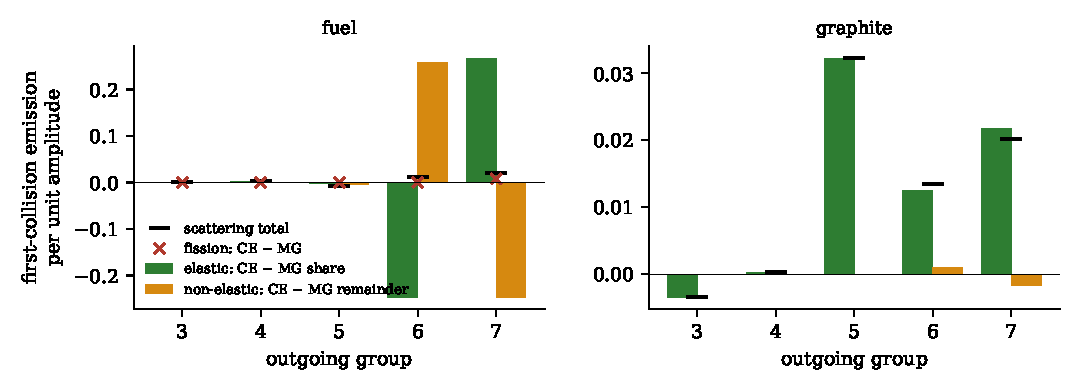
\includegraphics[width=0.92\textwidth]{figures/continuous_channels.pdf}
\caption{First-collision emission, CE minus multigroup, by outgoing group and channel class. The
multigroup matrix holds inelastic scattering; split by one elastic share per incident group, the
elastic and non-elastic parts of the fuel's fast groups differ by about $0.25$ with opposite signs,
and their sum is small.}\label{fig:cont:channels}
\end{figure}

\paragraph{The measure.} One generation's importance-weighted residual, with the importance tabulated
by field region and 60 energy bins, split into a \emph{bin part} (the residual's bin totals times the
bins' mean importance) and a \emph{within-bin part} (the rest), as noise per root second. The split
reproduces the ordering of the eigenvalue figures of merit: the control variate of
Section~\ref{sec:res:bcv} has bin part $0.0097$ (forward bins) and within-bin part $0.024$ (backward
records), $85\%$ of its variance (Figure~\ref{fig:cont:cvbins}).

\begin{figure}[t]\centering
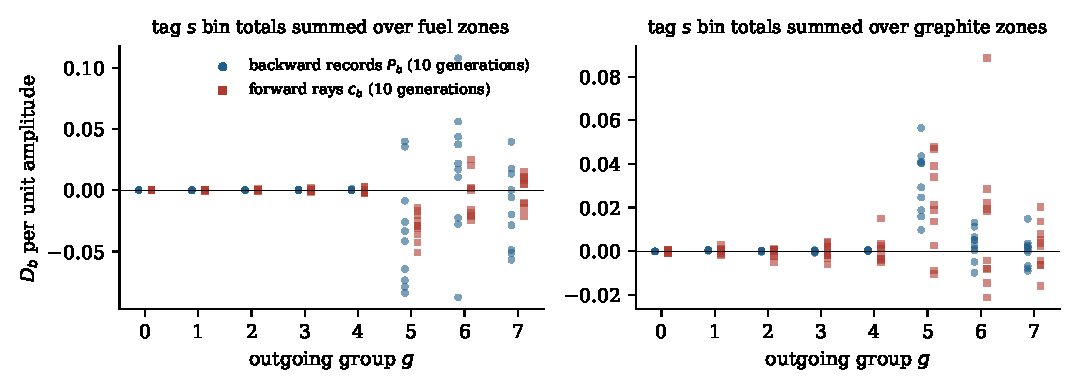
\includegraphics[width=0.92\textwidth]{figures/continuous_cv_bins.pdf}
\caption{Bin totals of the scattering residual's physics part over ten generations: backward records
(blue) and forward rays (red), summed over the zones of each material.}\label{fig:cont:cvbins}
\end{figure}

\paragraph{Partners.} The ray-wise mismatch $\rho=\E\!\int|k_{CE}-k_0|/\E\!\int k_{CE}$ sets the weights:
\begin{center}\footnotesize
\begin{tabular}{@{}lccc@{}}
\toprule
partner & lanes or bands & $\rho$ elastic & $\rho$ fission\\ \midrule
multigroup & 1 & 0.255 & 0.74\\
CE law applied to the multigroup flux & 1 & 0.125 & 0.153\\
RESOLVE lanes, generic starting block with the field's lifts & 64 & 0.017 & 0.033\\
RESOLVE lanes, starting block tuned to the problem & 32 & 0.002 & 0.003\\
bands (subgroup limit), $\log\Sigma_t$ levels, $128\times16$ & 2048 & 0.012 & 0.018\\
\bottomrule
\end{tabular}
\end{center}
The multigroup partner's floor is the in-group attenuation along the ray; RESOLVE lanes remove it.
Truncating the partner's angular law to P$_1$, P$_3$ or P$_7$ leaves $0.11$, $0.08$, $0.065$.

\paragraph{Bounded weights.} With the CE and multigroup proposals alone, $90\%$ of the variance sat in
$0.1\%$ of the samples, at the $^{238}$U resonance minima where the partner and CE disagree and neither
proposal puts mass. A third component drawn from a band library (band by source mass, collision with
the band's $\Sigma_t$, incident energy by $\Sigma_{el}$ within the band) bounds the weights of a band
partner. RESOLVE lanes ring with both signs at the resonance peaks and keep their tails.

\paragraph{Noise.} Scattering, per root second (total; within-bin): multigroup partner $0.119$; $0.028$;
band partner $128\times16$ with the band proposal $0.0064$; $0.0025$, at 20~$\mu$s per sample. Fission
with that partner: $0.0018$ (backward records $0.0098$).

\paragraph{The closure.} The partner's expectation must be added back. Its bin totals come from a band
first-flight sweep (\code{rmc.band\_sweep}: long random rays carry the uncollided flux in every band,
the local part of each segment integral replaced by its exact expectation) and elastic transfer
tables. Gate G8.17 checks them against the partner's own forward points. Its noise per root second is
$0.004$--$0.016$ depending on the number of bands, so that points plus closure total about $0.018$
($32\times16$ bands), against $0.034$ for the control variate: about $3.6$ times in variance $\times$
time, from one generation; the eigenvalue is not yet measured.

\paragraph{What remains.} With the multigroup field, the closure also has structure inside the bins
(the partner's exact-kinematics emission against the multigroup lift), which the points do not carry.
A band field, the band fluxes times tabulated CE emission spectra, removes the energy part; what
remains is the flat-source and angular structure, as for any low order.

\subsection{What optimization could recover}\label{sec:s8:projection}

\begin{table}[t]\centering\small
\caption{Time per generation of the tuned combined variant (single thread), and the projected
speedup of each kernel.}\label{tab:impl:time}
\begin{tabular}{@{}lrrrl@{}}
\toprule
kernel & s/gen & share & projected $\times$ & reason\\
\midrule
residual sampling & 1.55 & 49\% & 4 & total-only lookups, per-path XS cache, channel sampling\\
flights & 0.52 & 16\% & 1.5 & already OpenMC's own collision physics; bank I/O only\\
cancellation & 0.32 & 10\% & 5 & Python loops and \code{numpy} netting moved to C++\\
tallies and bookkeeping & 0.78 & 25\% & 5 & closed-form MG low, C++ bank handling\\
\midrule
total & 3.17 & & 3.3 & \\
\bottomrule
\end{tabular}
\end{table}

\paragraph{Engineering.} Table~\ref{tab:impl:time} splits a generation by kernel.

Residual sampling dominates, and within it the cross-section lookups on backward segments
(Section~\ref{sec:impl:projection}). Each lookup is a full \code{Material::calculate\_xs}, while the
backward flux needs only $\Sigma_t$. A total-only lookup with a per-path cache would remove most of
that cost.

The Python-side cancellation and tally costs are pure overhead.

The flights are OpenMC's own transport and gain little. With the per-kernel factors of the table, a
generation becomes $3.3$ times faster. The $k$ figure of merit would then be $0.07$ (batch means) or
$0.005$ (replicas) of the reference: still at least $15$ times worse than analog Monte Carlo.

\paragraph{Algorithm.} Engineering cannot close that gap, so the remaining factors must come from
the algorithm. The follow-up of Section~\ref{sec:res:followup} narrows down which ones matter.
\begin{enumerate}
\item \textbf{Less noise per residual sample.} This is the dominant lever. The scattering residual
  injects about 7 units of absolute weight per generation, almost all of it integration noise of the
  high term. The candidates are:
  \begin{itemize}
  \item stratified or randomized quasi-Monte Carlo incident directions;
  \item importance-sampled incident energies;
  \item a CE/MG control evaluated on the same incident energies, so that the difference is
    pointwise residual-scale.
  \end{itemize}
  More samples per generation help in the same way: at $N=16000$, $\Wabs$ falls to $1.8$ and the
  figure of merit rises by about two even before optimization (Table~\ref{tab:fu}). Cheaper samples
  (Table~\ref{tab:impl:time}) therefore pay twice.
\item \textbf{Lower $\Wabs$ at fixed noise.} Following amplitudes ($b=a$) remove the production-scale
  amplitude term (21\% lower $\Wabs$). Pooling of scattering children at birth against a shared
  slowing-down density is the remaining exact option.
\item \textbf{Not the correlation.} In neutron lifetimes the collision iteration is already less
  correlated than analog Monte Carlo. Fission-to-fission generations cost more than they save
  (Section~\ref{sec:res:followup}).
\end{enumerate}

\paragraph{Projection to a light-water pincell.} The answer above is for graphite. For a typical PWR
pincell (UO$_2$, water, pitch 1.26~cm), the changes are as follows.
\begin{itemize}
\item \textbf{Reference cost.} A history takes $\approx20$ collisions to thermalize in hydrogen
  ($\xi\approx0.93$), against $\approx115$ in carbon. The reference therefore runs $\approx4$--$5$
  times faster per history.
\item \textbf{RMC cost.} The RMC generation is one collision generation, so its cost per generation
  is unchanged.
\item \textbf{Correlation.} The scattering modes decay as $c^n$ with $c$ lower in a hydrogenous
  pincell (more absorption per collision near the fuel), so the correlation time shortens by a
  similar factor.
\item \textbf{Residual.} The MG field is a worse approximation in an LWR: harder spectrum, stronger
  $^{238}$U self-shielding, more epithermal fission. This raises $V_{res}$ and $\Wabs$.
\end{itemize}
The net is roughly neutral to unfavourable. The LWR figure of merit ratio should be no better than
the graphite one, and plausibly 2--3 times worse unless the MG field carries self-shielded
cross sections.

\subsection{Verdict}

The method runs, and after Sections~\ref{sec:res:speedup} and~\ref{sec:res:lifts} it is unbiased
within the present precision:
\begin{itemize}
\item \textbf{Bias.} With lifts that resolve the resonances, the eigenvalue bias is $-86\pm58$~pcm
  (nine replicas), down from $+650$ to $+1000$~pcm. Its cause was netting acting on the unresolved
  resonance structure of the low term.
\item \textbf{The correction.} The scattering residual is about 15 times more efficient than in the
  first measurement (proposal, tracer, several energies per trace, lifts). The bank's absolute
  weight is below the fission production ($\Wabs\approx0.85$), from 4.4.
\item \textbf{Figure of merit.} With the binned control variate of Section~\ref{sec:res:bcv}, whose
  residual is unbiased, it is $1$--$2$ times analog Monte Carlo's for $k$ on the spread of six
  replicas and $2$--$3$ on batch means; with residual samples from backward points it was about
  $0.4$. A biased form that holds the residual only in the netting bins reached $5.5$
  (Section~\ref{sec:res:correlated}). Pointwise forward points with a band partner and its closure
  project to about $3.6$ times the control variate (Section~\ref{sec:res:continuous}).
\end{itemize}

What limits it has changed three times. It is no longer the scattering residual, no longer the
field's fission production $X$ (Section~\ref{sec:res:X}), and no longer the eigenvalue update, whose
lifetime-long memory the balance estimate removes. Exact grouped cancellation at fission births is
implemented and verified, but it is not sufficient for weight cancellation: the weight that must
cancel is scattering weight, and netting remains necessary. The next stage should:
\begin{enumerate}
\item test a problem with fewer collisions per neutron lifetime (a water lattice or a fast system):
  a coarser mesh, a better loss estimator and a resonance-resolving low order have all left the
  figure of merit where it was on the graphite pincell (Section~\ref{sec:res:forward});
\item build a single-generation efficiency measure that includes netting, so that the sampler can be
  tuned again; and find the origin of the bias of $-10$ to $-50$~pcm.
\end{enumerate}

